% Options for packages loaded elsewhere
% Options for packages loaded elsewhere
\PassOptionsToPackage{unicode}{hyperref}
\PassOptionsToPackage{hyphens}{url}
\PassOptionsToPackage{dvipsnames,svgnames,x11names}{xcolor}
%
\documentclass[
  12pt,
  letterpaper,
  DIV=11,
  numbers=noendperiod]{scrartcl}
\usepackage{xcolor}
\usepackage[margin=2cm]{geometry}
\usepackage{amsmath,amssymb}
\setcounter{secnumdepth}{5}
\usepackage{iftex}
\ifPDFTeX
  \usepackage[T1]{fontenc}
  \usepackage[utf8]{inputenc}
  \usepackage{textcomp} % provide euro and other symbols
\else % if luatex or xetex
  \usepackage{unicode-math} % this also loads fontspec
  \defaultfontfeatures{Scale=MatchLowercase}
  \defaultfontfeatures[\rmfamily]{Ligatures=TeX,Scale=1}
\fi
\usepackage{lmodern}
\ifPDFTeX\else
  % xetex/luatex font selection
  \setmainfont[]{Nimbus Roman}
\fi
% Use upquote if available, for straight quotes in verbatim environments
\IfFileExists{upquote.sty}{\usepackage{upquote}}{}
\IfFileExists{microtype.sty}{% use microtype if available
  \usepackage[]{microtype}
  \UseMicrotypeSet[protrusion]{basicmath} % disable protrusion for tt fonts
}{}
\makeatletter
\@ifundefined{KOMAClassName}{% if non-KOMA class
  \IfFileExists{parskip.sty}{%
    \usepackage{parskip}
  }{% else
    \setlength{\parindent}{0pt}
    \setlength{\parskip}{6pt plus 2pt minus 1pt}}
}{% if KOMA class
  \KOMAoptions{parskip=half}}
\makeatother
% Make \paragraph and \subparagraph free-standing
\makeatletter
\ifx\paragraph\undefined\else
  \let\oldparagraph\paragraph
  \renewcommand{\paragraph}{
    \@ifstar
      \xxxParagraphStar
      \xxxParagraphNoStar
  }
  \newcommand{\xxxParagraphStar}[1]{\oldparagraph*{#1}\mbox{}}
  \newcommand{\xxxParagraphNoStar}[1]{\oldparagraph{#1}\mbox{}}
\fi
\ifx\subparagraph\undefined\else
  \let\oldsubparagraph\subparagraph
  \renewcommand{\subparagraph}{
    \@ifstar
      \xxxSubParagraphStar
      \xxxSubParagraphNoStar
  }
  \newcommand{\xxxSubParagraphStar}[1]{\oldsubparagraph*{#1}\mbox{}}
  \newcommand{\xxxSubParagraphNoStar}[1]{\oldsubparagraph{#1}\mbox{}}
\fi
\makeatother

\usepackage{color}
\usepackage{fancyvrb}
\newcommand{\VerbBar}{|}
\newcommand{\VERB}{\Verb[commandchars=\\\{\}]}
\DefineVerbatimEnvironment{Highlighting}{Verbatim}{commandchars=\\\{\}}
% Add ',fontsize=\small' for more characters per line
\usepackage{framed}
\definecolor{shadecolor}{RGB}{241,243,245}
\newenvironment{Shaded}{\begin{snugshade}}{\end{snugshade}}
\newcommand{\AlertTok}[1]{\textcolor[rgb]{0.68,0.00,0.00}{#1}}
\newcommand{\AnnotationTok}[1]{\textcolor[rgb]{0.37,0.37,0.37}{#1}}
\newcommand{\AttributeTok}[1]{\textcolor[rgb]{0.40,0.45,0.13}{#1}}
\newcommand{\BaseNTok}[1]{\textcolor[rgb]{0.68,0.00,0.00}{#1}}
\newcommand{\BuiltInTok}[1]{\textcolor[rgb]{0.00,0.23,0.31}{#1}}
\newcommand{\CharTok}[1]{\textcolor[rgb]{0.13,0.47,0.30}{#1}}
\newcommand{\CommentTok}[1]{\textcolor[rgb]{0.37,0.37,0.37}{#1}}
\newcommand{\CommentVarTok}[1]{\textcolor[rgb]{0.37,0.37,0.37}{\textit{#1}}}
\newcommand{\ConstantTok}[1]{\textcolor[rgb]{0.56,0.35,0.01}{#1}}
\newcommand{\ControlFlowTok}[1]{\textcolor[rgb]{0.00,0.23,0.31}{\textbf{#1}}}
\newcommand{\DataTypeTok}[1]{\textcolor[rgb]{0.68,0.00,0.00}{#1}}
\newcommand{\DecValTok}[1]{\textcolor[rgb]{0.68,0.00,0.00}{#1}}
\newcommand{\DocumentationTok}[1]{\textcolor[rgb]{0.37,0.37,0.37}{\textit{#1}}}
\newcommand{\ErrorTok}[1]{\textcolor[rgb]{0.68,0.00,0.00}{#1}}
\newcommand{\ExtensionTok}[1]{\textcolor[rgb]{0.00,0.23,0.31}{#1}}
\newcommand{\FloatTok}[1]{\textcolor[rgb]{0.68,0.00,0.00}{#1}}
\newcommand{\FunctionTok}[1]{\textcolor[rgb]{0.28,0.35,0.67}{#1}}
\newcommand{\ImportTok}[1]{\textcolor[rgb]{0.00,0.46,0.62}{#1}}
\newcommand{\InformationTok}[1]{\textcolor[rgb]{0.37,0.37,0.37}{#1}}
\newcommand{\KeywordTok}[1]{\textcolor[rgb]{0.00,0.23,0.31}{\textbf{#1}}}
\newcommand{\NormalTok}[1]{\textcolor[rgb]{0.00,0.23,0.31}{#1}}
\newcommand{\OperatorTok}[1]{\textcolor[rgb]{0.37,0.37,0.37}{#1}}
\newcommand{\OtherTok}[1]{\textcolor[rgb]{0.00,0.23,0.31}{#1}}
\newcommand{\PreprocessorTok}[1]{\textcolor[rgb]{0.68,0.00,0.00}{#1}}
\newcommand{\RegionMarkerTok}[1]{\textcolor[rgb]{0.00,0.23,0.31}{#1}}
\newcommand{\SpecialCharTok}[1]{\textcolor[rgb]{0.37,0.37,0.37}{#1}}
\newcommand{\SpecialStringTok}[1]{\textcolor[rgb]{0.13,0.47,0.30}{#1}}
\newcommand{\StringTok}[1]{\textcolor[rgb]{0.13,0.47,0.30}{#1}}
\newcommand{\VariableTok}[1]{\textcolor[rgb]{0.07,0.07,0.07}{#1}}
\newcommand{\VerbatimStringTok}[1]{\textcolor[rgb]{0.13,0.47,0.30}{#1}}
\newcommand{\WarningTok}[1]{\textcolor[rgb]{0.37,0.37,0.37}{\textit{#1}}}

\usepackage{longtable,booktabs,array}
\usepackage{calc} % for calculating minipage widths
% Correct order of tables after \paragraph or \subparagraph
\usepackage{etoolbox}
\makeatletter
\patchcmd\longtable{\par}{\if@noskipsec\mbox{}\fi\par}{}{}
\makeatother
% Allow footnotes in longtable head/foot
\IfFileExists{footnotehyper.sty}{\usepackage{footnotehyper}}{\usepackage{footnote}}
\makesavenoteenv{longtable}
\usepackage{graphicx}
\makeatletter
\newsavebox\pandoc@box
\newcommand*\pandocbounded[1]{% scales image to fit in text height/width
  \sbox\pandoc@box{#1}%
  \Gscale@div\@tempa{\textheight}{\dimexpr\ht\pandoc@box+\dp\pandoc@box\relax}%
  \Gscale@div\@tempb{\linewidth}{\wd\pandoc@box}%
  \ifdim\@tempb\p@<\@tempa\p@\let\@tempa\@tempb\fi% select the smaller of both
  \ifdim\@tempa\p@<\p@\scalebox{\@tempa}{\usebox\pandoc@box}%
  \else\usebox{\pandoc@box}%
  \fi%
}
% Set default figure placement to htbp
\def\fps@figure{htbp}
\makeatother


% definitions for citeproc citations
\NewDocumentCommand\citeproctext{}{}
\NewDocumentCommand\citeproc{mm}{%
  \begingroup\def\citeproctext{#2}\cite{#1}\endgroup}
\makeatletter
 % allow citations to break across lines
 \let\@cite@ofmt\@firstofone
 % avoid brackets around text for \cite:
 \def\@biblabel#1{}
 \def\@cite#1#2{{#1\if@tempswa , #2\fi}}
\makeatother
\newlength{\cslhangindent}
\setlength{\cslhangindent}{1.5em}
\newlength{\csllabelwidth}
\setlength{\csllabelwidth}{3em}
\newenvironment{CSLReferences}[2] % #1 hanging-indent, #2 entry-spacing
 {\begin{list}{}{%
  \setlength{\itemindent}{0pt}
  \setlength{\leftmargin}{0pt}
  \setlength{\parsep}{0pt}
  % turn on hanging indent if param 1 is 1
  \ifodd #1
   \setlength{\leftmargin}{\cslhangindent}
   \setlength{\itemindent}{-1\cslhangindent}
  \fi
  % set entry spacing
  \setlength{\itemsep}{#2\baselineskip}}}
 {\end{list}}
\usepackage{calc}
\newcommand{\CSLBlock}[1]{\hfill\break\parbox[t]{\linewidth}{\strut\ignorespaces#1\strut}}
\newcommand{\CSLLeftMargin}[1]{\parbox[t]{\csllabelwidth}{\strut#1\strut}}
\newcommand{\CSLRightInline}[1]{\parbox[t]{\linewidth - \csllabelwidth}{\strut#1\strut}}
\newcommand{\CSLIndent}[1]{\hspace{\cslhangindent}#1}



\setlength{\emergencystretch}{3em} % prevent overfull lines

\providecommand{\tightlist}{%
  \setlength{\itemsep}{0pt}\setlength{\parskip}{0pt}}



 


% Código
\usepackage{fvextra}
\DefineVerbatimEnvironment{Highlighting}{Verbatim}{
  breaklines=true,
  breakanywhere=true,
  commandchars=\\\{\}
}

% Interlineado ligeramente compacto
\usepackage{setspace}
\setstretch{1.05}

% Manejo de figuras
\usepackage{float}
\usepackage{placeins}
\KOMAoption{captions}{tableheading}
\makeatletter
\@ifpackageloaded{caption}{}{\usepackage{caption}}
\AtBeginDocument{%
\ifdefined\contentsname
  \renewcommand*\contentsname{Table of contents}
\else
  \newcommand\contentsname{Table of contents}
\fi
\ifdefined\listfigurename
  \renewcommand*\listfigurename{List of Figures}
\else
  \newcommand\listfigurename{List of Figures}
\fi
\ifdefined\listtablename
  \renewcommand*\listtablename{List of Tables}
\else
  \newcommand\listtablename{List of Tables}
\fi
\ifdefined\figurename
  \renewcommand*\figurename{Figure}
\else
  \newcommand\figurename{Figure}
\fi
\ifdefined\tablename
  \renewcommand*\tablename{Table}
\else
  \newcommand\tablename{Table}
\fi
}
\@ifpackageloaded{float}{}{\usepackage{float}}
\floatstyle{ruled}
\@ifundefined{c@chapter}{\newfloat{codelisting}{h}{lop}}{\newfloat{codelisting}{h}{lop}[chapter]}
\floatname{codelisting}{Listing}
\newcommand*\listoflistings{\listof{codelisting}{List of Listings}}
\makeatother
\makeatletter
\makeatother
\makeatletter
\@ifpackageloaded{caption}{}{\usepackage{caption}}
\@ifpackageloaded{subcaption}{}{\usepackage{subcaption}}
\makeatother
\usepackage{bookmark}
\IfFileExists{xurl.sty}{\usepackage{xurl}}{} % add URL line breaks if available
\urlstyle{same}
\hypersetup{
  colorlinks=true,
  linkcolor={blue},
  filecolor={Maroon},
  citecolor={Blue},
  urlcolor={Blue},
  pdfcreator={LaTeX via pandoc}}


\author{}
\date{}
\begin{document}

\begin{titlepage}

% Logos
\begin{minipage}{0.45\textwidth}
    \raggedright
    
\includegraphics[width=6.5cm]{data/images/Logo_UNAM.png}
\end{minipage}
\hfill
\begin{minipage}{0.45\textwidth}
    \raggedleft
    
\includegraphics[width=3.2cm]{data/images/Logo_LCG.png}
\end{minipage}

\vspace{1.5cm}

\begin{center}

{\Large Universidad Nacional Autónoma de México \par}
\vspace{0.3cm}

{\large Licenciatura en Ciencias Genómicas \par}
\vspace{1.5cm}

{\Huge \bfseries Proyecto Final \par}
\vspace{0.8cm}

{\Large Transcriptómica \par}

\vspace{2cm}

{\LARGE \bfseries
Análisis transcriptómico del envejecimiento cerebral en corteza prefrontal dorsolateral de \textit{Macaca mulatta}
\par}

\vspace{2cm}

{\large
Alumno: Mateo Jiménez Sotelo \par
Grupo: LCG22 \par
}

\vspace{1cm}

{\large
Docente: Dr. David Valle \par
}

\vfill

{\large
Semestre 2026-2 \par
Mayo 2026
}

\end{center}

\end{titlepage}


\section{Introducción}\label{introducciuxf3n}

\subsection{Planteamineto}\label{planteamineto}

El envejecimiento cerebral es un proceso biológico complejo asociado con
cambios progresivos en la expresión génica, la función neuronal y la
susceptibilidad a enfermedades neurodegenerativas. De esta forma,
diversos estudios transcriptómicos han mostrado que el envejecimiento se
acompaña de alteraciones en procesos relacionados con señalización
sináptica, inflamación, metabolismo energético y respuesta al estrés
celular. Sin embargo, gran parte de la información disponible presenta
limitaciones asociadas con diferencias fisiológicas, simplificación del
modelo o variabilidad experimental.

Los primates no humanos constituyen un modelo particularmente novedoso
para el estudio del envejecimiento cerebral por la conservación de
múltiples características humanas neuroanatómicas y fisiológicas. En
este contexto, el artículo
\href{https://www.nature.com/articles/s41593-022-01197-0\#Sec45}{\emph{Multiregion
transcriptomic profiling of the primate brain reveals signatures of
aging and the social environment}} {[}1{]} llevó a cabo un análisis
transcriptómico multirregional en cerebro de \emph{Macaca mulatta}
mediante RNA-seq, en el que se evaluaron asociaciones entre
\textbf{edad}, \textbf{ambiente social} y \textbf{expresión génica
cerebral}. Los datos utilizados en este proyecto fueron obtenidos del
\emph{bioproject} \texttt{PRJNA743289} y bajo el acceso
\textbf{GSE179330} en GEO.

A pesar de los avances en los estudios del fenómeno, aún existen
distintas limitaciones para comprender cómo es que el envejecimiento
afecta de manera coordinada distintos procesos celulares en el cerebro
de primates, y en consecuencia del macaco y, claro, del humano. En
concreto, gran parte de los estudios transcriptómicos en envejecimiento
cerebral se han realizado en modelos murinos o en tejidos humanos
\emph{post mortem}, los cuales presentan restricciones relacionadas con
divergencia evolutiva en el primer caso, y en general con variabilidad
individual y calidad del RNA recuperado en el segundo. Así, esto
dificulta la distinción entre cambios asociados al envejecimiento
fisiológico normal y vinculados más bien a procesos neurodegenerativos o
artefactos experimentales {[}1{]}.

La corteza prefrontal dorsolateral constituye una región de especial
interés debido a su participación en funciones cognitivas superiores
como memoria de trabajo, toma de decisiones y regulación conductual,
procesos que suelen deteriorarse progresivamente con la edad. Diversos
trabajos han reportado que el envejecimiento cerebral se acompaña de
alteraciones en vías relacionadas con metabolismo energético, respuesta
inflamatoria, comunicación sináptica y mantenimiento estructural
neuronal {[}1{]}. Sin embargo, la magnitud y dirección de estos cambios
puede variar considerablemente entre especies y regiones cerebrales, lo
que evidencia las falencias de utilizar ratones para extrapolar los
resultados a humano, al tiempo que resalta la relevancia de evaluar
estos patrones específicamente en modelos de primates evolutivamente
cercanos al \emph{Homo sapiens}.

Por lo anterior, se optó por analizar y procesar datos del estudio de
\emph{bulk} RNA-seq provenientes de \textbf{corteza prefrontal
dorsolateral} (dlPFC) de hembras jóvenes y adultas de \emph{Macaca
mulatta}. Se incluyen control de calidad de lecturas, limpieza de
adaptadores, alineamiento contra el genoma de referencia, cuantificación
de abundancias génicas y análisis de expresión diferencial mediante
\texttt{DESeq2}. Asimismo, se hicieron análisis funcionales de
enriquecimiento funcional utilizando \texttt{Gene\ Ontology},
\texttt{STRING} y \texttt{GSEA} en búsqueda de cambios de expresión
asociados con envejecimiento cerebral normal en dlPFC de macaco, para
evaluar si los patrones observados son consistentes con procesos
biológicos previamente reportados en estudios de envejecimiento cerebral
en primates.

\subsection{Objetivos}\label{objetivos}

\textbf{Objetivo general}

\begin{itemize}
\tightlist
\item
  Identificar cambios de expresión génica asociados con envejecimiento
  cerebral en corteza prefrontal dorsolateral de hembras de \emph{Macaca
  mulatta} mediante un \emph{pipeline} basado en RNA-seq.
\end{itemize}

\textbf{Objetivos específicos}

\begin{itemize}
\item
  Filtrar y seleccionar muestras de RNA-seq de \emph{Macaca mulatta}
  correspondientes a hembras jóvenes y adultas provenientes de dlPFC.
\item
  Evaluar y mejorar la calidad de las lecturas mediante herramientas de
  control de calidad y limpieza de secuencias.
\item
  Alinear las lecturas contra el genoma de referencia Mmul\_10
  utilizando alineadores de RNA-seq y cuantificar abundancias génicas.
\item
  Identificar genes diferencialmente expresados entre grupos de edad
  utilizando \texttt{DESeq2}.
\item
  Analizar procesos biológicos y rutas enriquecidas asociadas con los
  genes diferencialmente expresados mediante herramientas de
  enriquecimiento funcional y GSEA.
\item
  Interpretar los cambios transcriptómicos observados en el contexto
  biológico del envejecimiento cerebral en primates.
\end{itemize}

\section{Procedimiento y resultados}\label{procedimiento-y-resultados}

\begin{quote}
Los comandos pertenecientes a alineamientos y procesameinto posterior de
datos previo al análisis de expresión diferencial propiamente dicho, se
simplificaron en el cuerpo del reporte para no utilizar demasiado
espacio, pero se mantuvieron en el código fuente
(\texttt{./JimenezSotelo\_Mateo\_ProyectoFinal.qmd}) en la sección de
\textbf{Anexo}, al igual que los códigos de procesamiento o
\emph{parseo} de datos, para su consulta y reproducibilidad.
\end{quote}

\subsection{Datos}\label{datos}

\subsubsection{Metadatos}\label{metadatos}

Se descarga el archivo de \emph{metadata} \texttt{SraRunTable.csv}
mediante
\href{https://www.ncbi.nlm.nih.gov/Traces/study/?acc=PRJNA743289&o=acc_s\%3Aa}{SRA
Run Selector}. Este contiene 551 muestras secuenciadas con la plataforma
\emph{Illumina NovaSeq 6000} y 31 variables asociadas a metadatos, tanto
técnicos como biológicos.

\begin{verbatim}
Estructura: (551, 31)
Columnas:
\end{verbatim}

\begin{verbatim}
Instrument
Illumina NovaSeq 6000    551
Name: count, dtype: int64
\end{verbatim}

\begin{verbatim}
['Run', 'Assay Type', 'AvgSpotLen', 'Bases']
['BioProject', 'BioSample', 'Bytes', 'Center Name']
['Consent', 'DATASTORE filetype', 'DATASTORE provider', 'DATASTORE region']
['Experiment', 'GEO_Accession (exp)', 'Instrument', 'LibraryLayout']
['LibrarySelection', 'LibrarySource', 'Organism', 'Platform']
['ReleaseDate', 'create_date', 'version', 'Sample Name']
['SRA Study', 'AGE', 'individual_id', 'sex']
['source_name', 'tissue', 'Dominance_rank']
\end{verbatim}

\paragraph{Filtrado de muestras}\label{filtrado-de-muestras}

Con el objetivo de minimizar la heterogeneidad de los datos y maximizar
la potencia estadística, se opta por un filtrado de muestras
considerando aquellas correspondientes a datos de \emph{bulk RNA-seq}
\emph{paired-end} (PE) con las siguientes características:

\begin{itemize}
\tightlist
\item
  Sexo: \textbf{Femenino}
\item
  Edad: Grupos de \textbf{5 a 8} y de \textbf{12 a 16} años
\item
  Tejido: \textbf{corteza prefrontal dorsolateral} (dlPFC)
\end{itemize}

\begin{Shaded}
\begin{Highlighting}[]
\CommentTok{\# Solo dlPFC PE y hembras}
\NormalTok{dlpfc\_f }\OperatorTok{=}\NormalTok{ metadata[}
\NormalTok{  (metadata[}\StringTok{"tissue"}\NormalTok{] }\OperatorTok{==} \StringTok{"dorsolateral prefrontal cortex"}\NormalTok{) }\OperatorTok{\&}
\NormalTok{  (metadata[}\StringTok{"LibraryLayout"}\NormalTok{] }\OperatorTok{==} \StringTok{"PAIRED"}\NormalTok{) }\OperatorTok{\&}
\NormalTok{  (metadata[}\StringTok{"sex"}\NormalTok{] }\OperatorTok{==} \StringTok{"female"}\NormalTok{)}
\NormalTok{  ]}

\CommentTok{\# Filtrado por edad}
\NormalTok{young }\OperatorTok{=}\NormalTok{ dlpfc\_f[(dlpfc\_f[}\StringTok{"AGE"}\NormalTok{] }\OperatorTok{\textgreater{}=} \DecValTok{5}\NormalTok{) }\OperatorTok{\&}\NormalTok{ (dlpfc\_f[}\StringTok{"AGE"}\NormalTok{] }\OperatorTok{\textless{}=} \DecValTok{8}\NormalTok{)]}
\NormalTok{old }\OperatorTok{=}\NormalTok{ dlpfc\_f[(dlpfc\_f[}\StringTok{"AGE"}\NormalTok{] }\OperatorTok{\textgreater{}=} \DecValTok{12}\NormalTok{) }\OperatorTok{\&}\NormalTok{ (dlpfc\_f[}\StringTok{"AGE"}\NormalTok{] }\OperatorTok{\textless{}=} \DecValTok{16}\NormalTok{)]}
\end{Highlighting}
\end{Shaded}

\begin{verbatim}
Número de muestras jóvenes únicas: 8
\end{verbatim}

\begin{verbatim}
Número de muestras adultas únicas: 5
\end{verbatim}

\paragraph{Selección de muestras}\label{selecciuxf3n-de-muestras}

Tras el filtrado, se mantuvieron 13 muestras de IDs únicos (8 jóvenes y
5 adultas) derivadas de la misma plataforma y \emph{batch}, con un
\emph{Average Spot Length} de 202 bp. De estas, se seleccionaron 10 (5
jóvenes y las 5 adultas) para análisis posteriores, con base en la
cantidad de bases secuenciadas y buscando diversidad de edades.
Consecuentemente, se eligen las muestras con mayor profundidad de
secuenciación dentro del subconjunto sobrerrepresentado de 6 años.

\begin{Shaded}
\begin{Highlighting}[]
\CommentTok{\# Se separan muestras de 6 años y las demás}
\NormalTok{young\_6 }\OperatorTok{=}\NormalTok{ young[young[}\StringTok{"AGE"}\NormalTok{].astype(}\BuiltInTok{int}\NormalTok{) }\OperatorTok{==} \DecValTok{6}\NormalTok{]}
\NormalTok{young\_non6 }\OperatorTok{=}\NormalTok{ young.drop(young\_6.index)}

\CommentTok{\# Se seleccionan las 2 con más bases}
\NormalTok{young\_6\_selected }\OperatorTok{=}\NormalTok{ young\_6.sort\_values(}\StringTok{"Bases"}\NormalTok{, ascending}\OperatorTok{=}\VariableTok{False}\NormalTok{).head(}\DecValTok{2}\NormalTok{)}

\CommentTok{\# Conjunto joven final}
\NormalTok{young\_final }\OperatorTok{=}\NormalTok{ pd.concat([young\_non6, young\_6\_selected]).sort\_values(}\StringTok{"AGE"}\NormalTok{)}
\CommentTok{\# Conjunto total final}
\NormalTok{final\_samples }\OperatorTok{=}\NormalTok{ pd.concat([young\_final, old]).sort\_values(}\StringTok{"AGE"}\NormalTok{)}

\CommentTok{\# Columna de grupo de edad}
\CommentTok{\# Young...}
\NormalTok{final\_samples[}\StringTok{"AGE\_group"}\NormalTok{] }\OperatorTok{=} \StringTok{"young"}
\CommentTok{\# ...a menos que se vea lo contrario}
\NormalTok{final\_samples.loc[final\_samples[}\StringTok{"AGE"}\NormalTok{] }\OperatorTok{\textgreater{}=} \DecValTok{12}\NormalTok{, }\StringTok{"AGE\_group"}\NormalTok{] }\OperatorTok{=} \StringTok{"old"}

\CommentTok{\# Exportar metadata filtrada y lista de SRR a descargar}
\NormalTok{os.makedirs(}\StringTok{"./data/metadata"}\NormalTok{, exist\_ok}\OperatorTok{=}\VariableTok{True}\NormalTok{)}
\NormalTok{final\_samples.to\_csv(}\StringTok{"./data/metadata/selected\_samples.tsv"}\NormalTok{, sep}\OperatorTok{=}\StringTok{"}\CharTok{\textbackslash{}t}\StringTok{"}\NormalTok{, index}\OperatorTok{=}\VariableTok{False}\NormalTok{)}
\NormalTok{final\_samples[}\StringTok{"Run"}\NormalTok{].to\_csv(}\StringTok{"./data/metadata/srr\_ids.txt"}\NormalTok{, index}\OperatorTok{=}\VariableTok{False}\NormalTok{, header}\OperatorTok{=}\VariableTok{False}\NormalTok{)}
\end{Highlighting}
\end{Shaded}

\begin{quote}
Tabla y lista de muestras se encuentran en \texttt{./data/metadata/}.
\end{quote}

De esta manera, se descargan los siguientes SRR:

\begin{verbatim}
['SRR15024177', 'SRR15024188', 'SRR15024183', 'SRR15024186', 'SRR15024175']
['SRR15024178', 'SRR15024173', 'SRR15024174', 'SRR15024182', 'SRR15024168']
\end{verbatim}

\subsubsection{Descarga de datos}\label{descarga-de-datos}

Se descargan los 10 \emph{SRR}s seleccionados utilizando
\href{https://github.com/ncbi/sra-tools/wiki/HowTo:-fasterq-dump}{\texttt{fasterq-dump}}
de la \emph{suite} de herramientas SRA {[}2{]}, con 8 núcleos y
dividiendo los archivos en pares (PE). Posteriormente, se comprimen con
\texttt{gzip} para optimizar almacenamiento.

\subsubsection{Calidad y limpieza de
datos}\label{calidad-y-limpieza-de-datos}

Se evalúa la calidad de los \texttt{fastq}s descargados con
\href{https://www.bioinformatics.babraham.ac.uk/projects/fastqc/}{FastQC}
{[}3{]} y se visualiza el resumen de los resultados con
\href{http://dx.doi.org/10.1093/bioinformatics/btw354}{MultiQC} {[}4{]}
para decidir una estrategia de limpieza homogénea para todas las
muestras mediante el script \texttt{./scripts/clean\_fastqs.sh} y
utilizando 4 núcleos.

Las lecturas presentan una alta calidad global, teniendo un
\emph{Phred-score} consistentemente superior a 30 y contando todas con
una longitud de 101 bp (consistente con el \emph{Average Spot Length}
para PE reportado en los metadatos). Aún así, se detectó un leve
contenido de adaptadores hacia los extremos 3' de las lecturas, así como
un contenido de \emph{GC} discrepante del esperado teórico y niveles
moderados de secuencias sobre-representadas y duplicadas.

\begin{figure}[H]

{\centering \pandocbounded{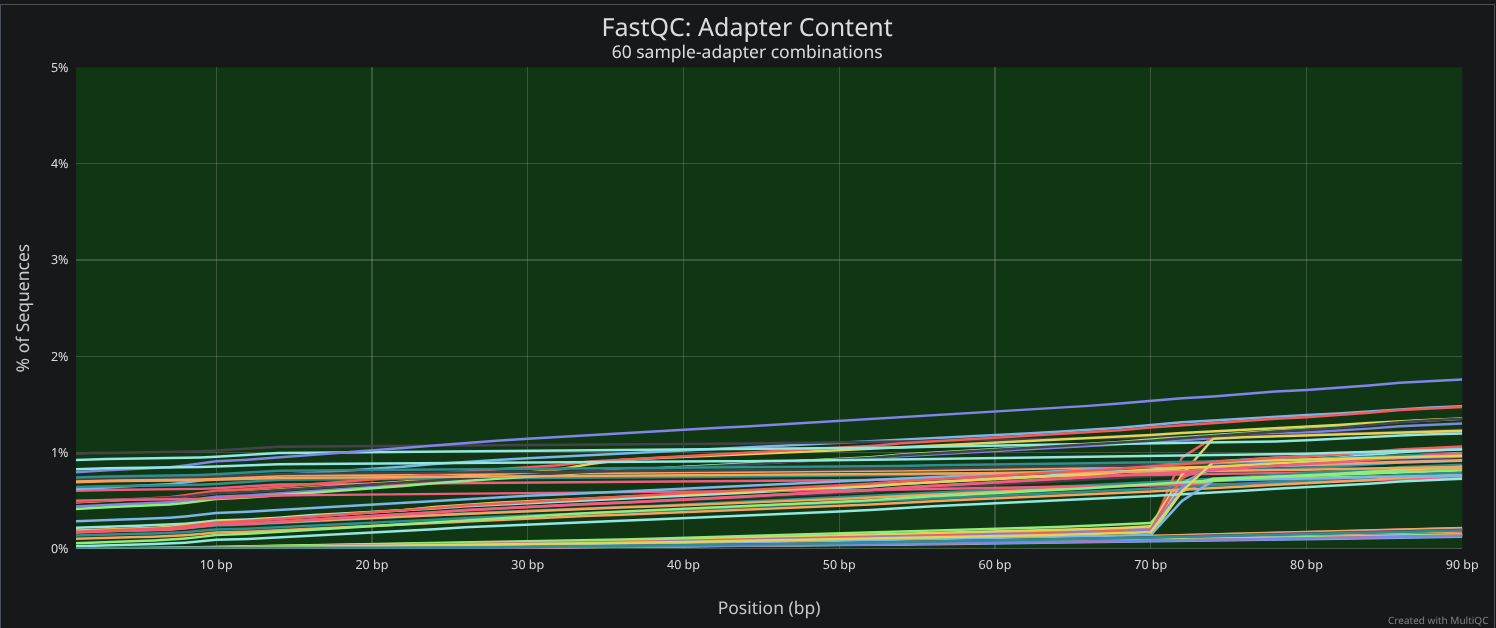
\includegraphics[keepaspectratio]{./data/images/multiqc/multiqc_adapter_content_raw.png}}

}

\caption{Contenido de adaptadores de las muestras previas a la limpieza}

\end{figure}%

Salvo la presencia de adaptadores, estas características son esperables
en datos de \emph{bulk RNA-seq} y no repercuten negativamente en
análisis posteriores {[}5{]}. Por esto, se opta limpiar adaptadores y
filtrar lecturas de baja calidad, sin eliminar secuencias
sobre-representadas o duplicadas.

La limpieza se lleva a cabo con
\href{https://pmc.ncbi.nlm.nih.gov/articles/PMC6129281/}{\texttt{fastp}}
{[}6{]} por igual en todas las muestras, con el fin de no introducir
ruido por un procesamiento heterogéneo. Se emplean detección automática
de adaptadores, \emph{trimming} de colas con baja calidad, eliminación
de artefactos \emph{polyG} y descarte de lecturas cortas (\textless50
bp) tras el \emph{trimming} para evitar alineamientos inespecíficos.
Esto se realiza mediante \texttt{./scripts/fastp\_per\_pe\_sample.sh}.

\begin{quote}
Se utilizan 8 núcleos y se generan reportes individuales en formato JSON
y HTML para cada muestra, almacenanados en \texttt{./data/cleaned/}
junto con los \texttt{fastq}s limpios.
\end{quote}

\begin{Shaded}
\begin{Highlighting}[]
\VariableTok{RAW\_PATH}\OperatorTok{=}\StringTok{"./data/raw"}
\VariableTok{CLEANED\_PATH}\OperatorTok{=}\StringTok{"./data/cleaned"}
\FunctionTok{mkdir} \AttributeTok{{-}p} \StringTok{"}\VariableTok{$\{CLEANED\_PATH\}}\StringTok{"}

\ExtensionTok{conda}\NormalTok{ activate fastp}

\ControlFlowTok{for}\NormalTok{ file }\KeywordTok{in} \VariableTok{$\{RAW\_PATH\}}\NormalTok{/SRR}\PreprocessorTok{*}\NormalTok{\_1.fastq.gz}\KeywordTok{;} \ControlFlowTok{do}
  \VariableTok{srr}\OperatorTok{=}\VariableTok{$(}\FunctionTok{basename} \StringTok{"}\VariableTok{$file}\StringTok{"}\NormalTok{ \_1.fastq.gz}\VariableTok{)} \CommentTok{\# Solo el SRR}

  \VariableTok{BASE\_RAW}\OperatorTok{=}\StringTok{"}\VariableTok{$\{RAW\_PATH\}}\StringTok{/}\VariableTok{$\{srr\}}\StringTok{"}
  \VariableTok{BASE\_CLEANED}\OperatorTok{=}\StringTok{"}\VariableTok{$\{CLEANED\_PATH\}}\StringTok{/}\VariableTok{$\{srr\}}\StringTok{"}

  \CommentTok{\# Paired End}
  \ExtensionTok{fastp} \DataTypeTok{\textbackslash{}}
    \AttributeTok{{-}i} \StringTok{"}\VariableTok{$\{BASE\_RAW\}}\StringTok{\_1.fastq.gz"} \AttributeTok{{-}I} \StringTok{"}\VariableTok{$\{BASE\_RAW\}}\StringTok{\_2.fastq.gz"} \DataTypeTok{\textbackslash{}}
    \AttributeTok{{-}o} \StringTok{"}\VariableTok{$\{BASE\_CLEANED\}}\StringTok{\_1.cleaned.fastq.gz"} \DataTypeTok{\textbackslash{}}
    \AttributeTok{{-}O} \StringTok{"}\VariableTok{$\{BASE\_CLEANED\}}\StringTok{\_2.cleaned.fastq.gz"} \DataTypeTok{\textbackslash{}}
    \AttributeTok{{-}{-}detect\_adapter\_for\_pe} \AttributeTok{{-}{-}trim\_poly\_g} \DataTypeTok{\textbackslash{}}
    \AttributeTok{{-}{-}cut\_tail} \AttributeTok{{-}{-}length\_required}\NormalTok{ 50 }\AttributeTok{{-}{-}thread}\NormalTok{ 8 }\DataTypeTok{\textbackslash{}}
    \AttributeTok{{-}{-}json} \StringTok{"}\VariableTok{$\{CLEANED\_PATH\}}\StringTok{/}\VariableTok{$\{srr\}}\StringTok{.json"} \DataTypeTok{\textbackslash{}}
    \AttributeTok{{-}{-}html} \StringTok{"}\VariableTok{$\{CLEANED\_PATH\}}\StringTok{/}\VariableTok{$\{srr\}}\StringTok{.html"}
\ControlFlowTok{done}

\ExtensionTok{conda}\NormalTok{ deactivate}
\end{Highlighting}
\end{Shaded}

Una vez limpios, se reutiliza \texttt{./scripts/clean\_fastqs.sh} para
evaluar la calidad de los \texttt{fastq}s procesados.

Se observa que la longitud de las lecturas ahora ya no es la misma a lo
largo de las muestras, lo cual es esperado dado el \emph{trimming} y la
remoción de adaptadores. En cambio, el contenido de adaptadores
disminuye al tiempo que el \emph{Phred-score} se mantiene alto.

\begin{figure}[H]

{\centering \pandocbounded{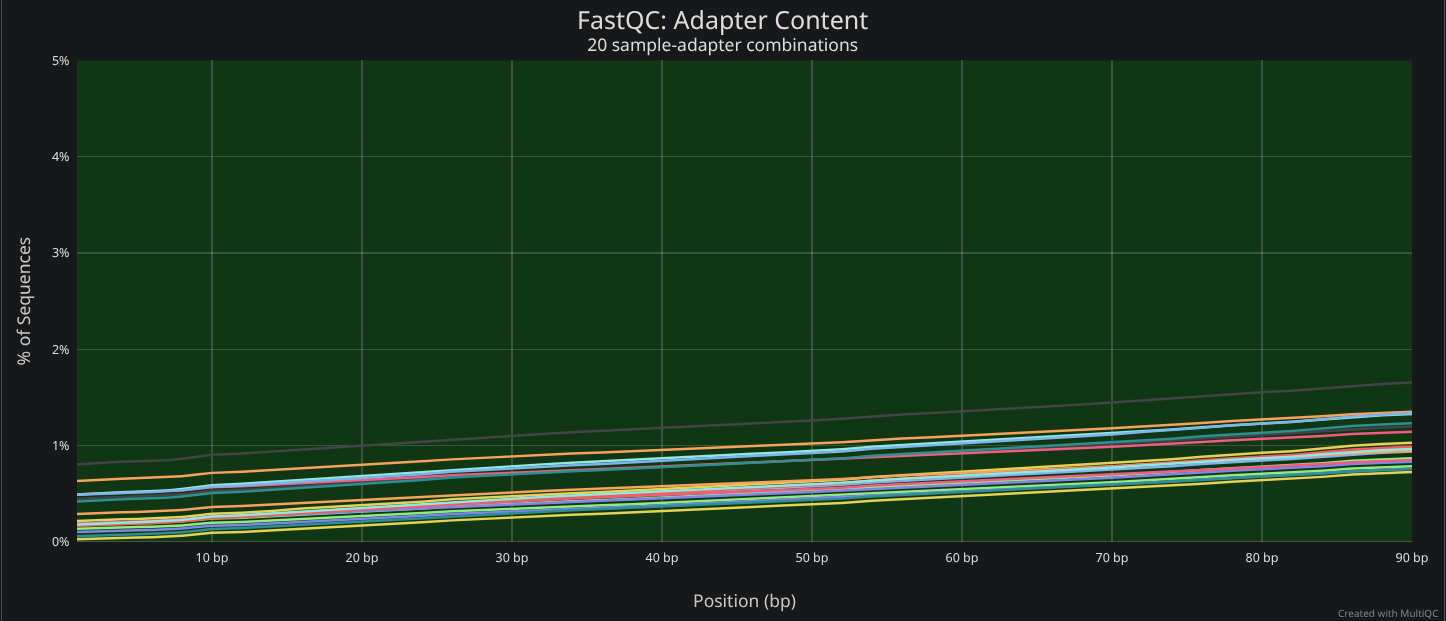
\includegraphics[keepaspectratio]{./data/images/multiqc/multiqc_adapter_content_cleaned.png}}

}

\caption{Contenido de adaptadores de las muestras tras la limpieza}

\end{figure}%

\subsection{Alineamientos}\label{alineamientos}

Se utilizaron los alineadores \texttt{STAR} {[}7{]} y \texttt{HISAT2}
{[}8{]}, que \emph{indexan} con base en un genoma de referencia provisto
para mapear las lecturas. Dada la disponibilidad de recursos en el
servidor \texttt{chaac}, suficientes para correr alineamientos
tradicionales, y a la capacidad de estos de recuperar información
posicional de las lecturas, útil para visualizaciones a nivel genómico,
se optó por \textbf{no hacer} \emph{pseudoalineamientos}.

Para la construcción de los índices de referencia de cada alineador, se
utilizaron el genoma de referencia \textbf{Mmul\_10} de \emph{Macaca
mulatta} \textbf{Release 115}
(\texttt{./data/references/Macaca\_mulatta.Mmul\_10.dna.toplevel.fa}) y
el GTF de anotación correspondiente
(\texttt{./data/references/Macaca\_mulatta.Mmul\_10.115.gtf}). Ambos se
obtuvieron de
\href{https://www.ensembl.org/Macaca_mulatta/Info/Index}{Ensembl}
{[}9{]}.

El índice de STAR se construyó utilizando
\texttt{-\/-sjdbOverhang\ 100}, correspondiente a la longitud de lectura
menos uno para lecturas PE de 101 bp. Este parámetro permite optimizar
el mapeo de lecturas que abarcan uniones exón-exón al incorporar
secuencias flanqueantes alrededor de los \emph{splice junctions}
anotados en el GTF de referencia {[}7{]}.

Para el alineamiento con \texttt{STAR} se generaron directamente
archivos BAM y conservaron las lecturas no alineadas mediante
\texttt{./scripts/star\_align.sh}

\begin{Shaded}
\begin{Highlighting}[]
\VariableTok{SRR}\OperatorTok{=}\VariableTok{$1}
\VariableTok{DATA}\OperatorTok{=}\StringTok{"./data/cleaned"}
\VariableTok{OUT}\OperatorTok{=}\StringTok{"./results/aligned/star\_}\VariableTok{$\{MODE\}}\StringTok{"}
\VariableTok{INDEX}\OperatorTok{=}\VariableTok{$2}
\VariableTok{LOG\_DIR}\OperatorTok{=}\StringTok{"./logs/STAR"}

\ExtensionTok{conda}\NormalTok{ activate star}

\VariableTok{INPUT}\OperatorTok{=}\StringTok{"}\VariableTok{$\{DATA\}}\StringTok{/}\VariableTok{$\{SRR\}}\StringTok{\_1.cleaned.fastq.gz }\VariableTok{$\{DATA\}}\StringTok{/}\VariableTok{$\{SRR\}}\StringTok{\_2.cleaned.fastq.gz"}

\CommentTok{\# Incluye reads mapeados y no mapeados en el bam}
\ExtensionTok{/usr/bin/time} \AttributeTok{{-}v}\NormalTok{ STAR }\DataTypeTok{\textbackslash{}}
  \AttributeTok{{-}{-}genomeDir} \VariableTok{$INDEX} \DataTypeTok{\textbackslash{}}
  \AttributeTok{{-}{-}readFilesIn} \VariableTok{$\{INPUT\}} \DataTypeTok{\textbackslash{}}
  \AttributeTok{{-}{-}readFilesCommand}\NormalTok{ zcat }\DataTypeTok{\textbackslash{}}
  \AttributeTok{{-}{-}runThreadN}\NormalTok{ 8 }\DataTypeTok{\textbackslash{}}
  \AttributeTok{{-}{-}outFileNamePrefix} \VariableTok{$\{OUT\}}\NormalTok{/}\VariableTok{$\{SRR\}}\NormalTok{\_ }\DataTypeTok{\textbackslash{}}
  \AttributeTok{{-}{-}outSAMtype}\NormalTok{ BAM SortedByCoordinate }\DataTypeTok{\textbackslash{}}
  \AttributeTok{{-}{-}outSAMunmapped}\NormalTok{ Within }\DataTypeTok{\textbackslash{}}
  \DecValTok{2}\OperatorTok{\textgreater{}\textgreater{}} \VariableTok{$\{LOG\_DIR\}}\NormalTok{/}\VariableTok{$\{SRR\}}\NormalTok{\_time.log}

\ExtensionTok{conda}\NormalTok{ deactivate}
\end{Highlighting}
\end{Shaded}

\subsubsection{HISAT2}\label{hisat2}

Se corrieron ambos alineadores para todas las muestras descargadas como
\emph{job}s independientes y se guardan los archivos \texttt{BAM}
resultantes del \emph{output} o derivados del mismo, en el caso de
\texttt{HISAT2}.

Debido a que ambos alineadores recuperaron un número similar de lecturas
mapeadas y a que \texttt{STAR}, si bien computacionalmente más pesado,
presentó una mayor tasa de mapeo único que \texttt{HISAT2}, se optó por
reportar únicamente los resultados de \texttt{STAR} en los análisis
posteriores, aunque los obtenidos con \texttt{HISAT2} se mantienen
disponibles para su consulta y comparación en la sección de
\textbf{Anexo}.

\subsection{Filtrado}\label{filtrado}

Se utilizó \texttt{samtools} ({[}10{]}) para filtrar los archivos
\texttt{BAM}, de forma que solo queden los alineamientos con
\emph{Mapping quality} \(\geq 10\) (\emph{E-value} \textgreater{} 0.1),
el cual es considerado el umbral estándar en \emph{pipelines} de
transcriptómica {[}5{]}. Posteriormente, los alineamientos se ordenaron
por coordenada genómica e indexaron para optimizar su lectura y
navegación, usando la \emph{flag} \texttt{-f\ 64} para contar solo la
primera lectura del par \emph{PE}. Los archivos recibieron el sufijo
\texttt{\_fs} para denotar \emph{filtered and sorted}.

\subsection{Cuantificación de
abundancias}\label{cuantificaciuxf3n-de-abundancias}

Se obtuvo el conteo de lecturas por gen a partir de los \texttt{BAM} con
\texttt{featureCounts}, del paquete \texttt{Subread} {[}11{]}, y el
\emph{GTF} descargado de forma previa. Se probó el parámetro de
\emph{strandness} \texttt{-s} tanto en \emph{forward} (1) como en
\emph{reverse} (2) para evaluar la dirección de las lecturas en la
librería, pero dado que las tasas de mapeo decayeron a valores promedio
de 38.38\% y 37.80\%, respectivamente, se optó por usar \texttt{-s\ 0},
sin asumir direccionalidad, consiguiendo tasas de mapeo de 71.87\%.
Adicionalmente, se contabilizaron solo los pares correctamente
alineados, cuantificaron los fragmentos completos en lugar de lecturas
individules y resolvieron ambigüedades asignando cada fragmento al gen
con el mayor solapamiento.

\begin{Shaded}
\begin{Highlighting}[]
\ExtensionTok{conda}\NormalTok{ activate subread}

\CommentTok{\# Comando con medición de tiempo y recursos}
\ExtensionTok{/usr/bin/time} \AttributeTok{{-}v}\NormalTok{ featureCounts }\DataTypeTok{\textbackslash{}}
  \AttributeTok{{-}o} \StringTok{"}\VariableTok{$\{BAM\_PATH\}}\StringTok{/counts\_per\_gene\_}\VariableTok{$\{STRAND\}}\StringTok{.txt"} \DataTypeTok{\textbackslash{}}
  \AttributeTok{{-}T}\NormalTok{ 8 }\DataTypeTok{\textbackslash{}}
  \AttributeTok{{-}a} \StringTok{"}\VariableTok{$\{GTF\}}\StringTok{"} \DataTypeTok{\textbackslash{}}
  \AttributeTok{{-}{-}largestOverlap} \DataTypeTok{\textbackslash{}}
  \AttributeTok{{-}p} \AttributeTok{{-}B} \AttributeTok{{-}s} \VariableTok{$\{STRAND\}} \DataTypeTok{\textbackslash{}}
  \AttributeTok{{-}{-}countReadPairs} \DataTypeTok{\textbackslash{}}
  \StringTok{"}\VariableTok{$\{BAM\_PATH\}}\StringTok{"}\NormalTok{/}\PreprocessorTok{*}\NormalTok{fs.bam }\DataTypeTok{\textbackslash{}}
  \DecValTok{2}\OperatorTok{\textgreater{}\textgreater{}} \StringTok{"}\VariableTok{$\{LOG\}}\StringTok{"}

\ExtensionTok{conda}\NormalTok{ deactivate}
\end{Highlighting}
\end{Shaded}

\subsection{Matrices de conteos}\label{matrices-de-conteos}

Las matrices de conteos obtenidas con \texttt{featureCounts} se
\emph{reformatearon} con \texttt{./scripts/homogenize\_matrixes.py} para
ser compatibles con los programas de análisis de expresión diferencial,
eliminando así los metadatos y ordenando las muestras en las columnas y
los genes en las filas. Las matrices se guardaron en formato
\texttt{tsv} en \texttt{./results/DEG/count\_matrices/} y cuentan con 10
columnas, correspondientes a las 5 muestras de cada condición, y 35,432
filas, correspondientes a los genes comunes entre ambas matrices.

\subsection{Anotaciones y archivos
auxiliares}\label{anotaciones-y-archivos-auxiliares}

A partir del archivo GTF se derivaron una tabla de correspondencia entre
\texttt{gene\_id} y \texttt{gene\_name}, útil para la identificación de
genes, y una tabla de anotación de longitudes génicas, para el cálculo
de métricas normalizadas. La primera tabla encontró equivalencias para
24,482 genes pues no todos los \texttt{gene\_id} presentes en la matriz
de conteos poseen una anotación de \texttt{gene\_name} asociada en el
GTF de \emph{Ensembl} para \emph{Macaca mulatta}. Esto posiblemente se
deba a diferencias en la calidad de las anotaciones con respecto a
organismos más estudiados pero no afecta los análisis posteriores, ya
que los conteos se conservaron utilizando los \texttt{gene\_id}s.

\subsection{Condiciones}\label{condiciones}

Se derivó una \textbf{tabla de condiciones} para cada muestra
seleccionada a partir de los metadatos ya filtrados por sexo, tejido y
edad (\texttt{./data/metadata/selected\_samples.tsv}), con la condición
en el formato \texttt{f\_\textless{}group\textgreater{}} y el mismo
número y orden de filas que las columnas de la matriz de conteos
\texttt{./results/DEG/count\_matrices/star\_PE\_counts.tsv}, de modo que
los algoritmos de \emph{DE} puedan asociar correctamente cada muestra
con su información correspondiente {[}5{]}.

\begin{table}[H]

\caption{\label{tbl-samples-order}Orden de las muestras en la tabla de
condiciones. Las muestras no se encuentran ordenadas por condición, sino
que siguen el orden alfabético de las matrices de conteos. Los
algoritmos de DE asocian cada muestra con su condición según el orden de
las filas, y este se mantiene consistente, por lo que la estrategia de
ordenado es indistinta.}

\centering{

\begin{verbatim}
        sample condition
0  SRR15024168     f_old
1  SRR15024173     f_old
2  SRR15024174     f_old
3  SRR15024175   f_young
4  SRR15024177   f_young
5  SRR15024178     f_old
6  SRR15024182     f_old
7  SRR15024183   f_young
8  SRR15024186   f_young
9  SRR15024188   f_young
\end{verbatim}

}

\end{table}%

\subsection{Expresión diferencial}\label{expresiuxf3n-diferencial}

El análisis de expresión diferencial se llevó a cabo en \texttt{R} con
\texttt{DESeq2} {[}12{]} y \texttt{edgeR} {[}13{]}, utilizando las
matrices de conteos y las tablas de condiciones. Se usó un diseño simple
con la condición de grupo de edad como única variable. Además, se
consideraron como genes diferencialmente expresados (DEG) aquellos con
un \emph{adjusted p-value} \textless{} 0.05 y un valor absoluto de
\emph{log2 fold change} \textgreater{} 0.5, debido a que pruebas
exploratorias previas con umbrales más estrictos apenas capturaban DEG.

Se utilizó el diseño \(~ 0 + condition\) para modelar la expresión
génica sin intercepto, permitiendo comparar las condiciones de forma
explícita sin establecer ninguna condición de referencia. Este diseño
facilita la interpretación de los resultados al los coeficientes del
modelo corresponder directamente a cada condición, en lugar de a la
diferencia respecto a una condición de referencia {[}5,14{]}.

El análisis se llevó a cabo mediante un \emph{pipeline} generalizado a
ambos algortimos, homogenizando aquellas funciones reutilizables entre
estos, manteniendo consistencia sintáctica entre las que no, y
conservando los mismos parámetros estadísticos y criterios de
significancia. Este consiste en los siguientes pasos:

\begin{enumerate}
\def\labelenumi{\arabic{enumi}.}
\tightlist
\item
  Cargado de matriz de conteos asociada.
\item
  Construcción del objeto estadístico correspondiente
  (\texttt{DESeqDataSet} o \texttt{DGEList}).
\item
  Filtrado de genes con baja expresión.
\item
  Análisis exploratorio mediante PCA.
\item
  Normalización y modelado de dispersión.
\item
  Transformación de matrices para análisis exploratorio.
\item
  Ajuste de un modelo \emph{binomial negativo} con diseño
  \texttt{\textasciitilde{}\ 0\ +\ condition}
\item
  Contrastes entre muestras de \textbf{5 a 8} y de \textbf{12 a 16}
  años.
\item
  Extracción de los DEG.
\item
  Visualización de resultados mediante \emph{volcano plots} y
  \emph{heatmaps}.
\end{enumerate}

Debido a que \texttt{DESeq2} posee una integración más directa con las
estrategias de visualización y normalización vistas durante el curso
{[}5,14{]} y dado que ambos métodos recuperaron patrones globales de
separación entre condiciones y DEG heterogéneos pero aún concordantes
entre sí, se decidió reportar solamente sus resultados en el cuerpo del
documento. Las estrategias seguidas y resultados completos de
\texttt{edgeR} se incluyen en la sección de \textbf{Anexo} para fines de
comparación y reproducibilidad.

A continuación se explican las decisiones tomadas en cada uno de los
pasos del \emph{pipeline}:

\begin{quote}
Los códigos de las funciones no incluidas se encuentran en la sección de
\textbf{Anexo}
\end{quote}

\begin{itemize}
\item
  \textbf{Filtrado de genes}: El filtrado de genes con baja expresión se
  hizo con la función \texttt{filterByExpr}, que es nativa de
  \texttt{edgeR} pero se utilizó en ambos casos para mantener criterios
  de filtrado consistentes entre los métodos {[}5,14{]}.
\item
  \textbf{PCA exploratorio}: Para el PCA, pese a que existen métodos
  específicos en cada algoritmo para generarlo, como \texttt{vst}, en el
  caso de \texttt{DESeq2}, se optó por utilizar de forma generalizada la
  función \texttt{prcomp} del paquete \texttt{stats} de \texttt{R} base.
  Esta toma la matriz de conteos transformada y normalizada y usa los
  mismos criterios de visualización para mantener la comparabilidad
  entre los métodos. El \emph{ploteo} se realizó mediante
  \texttt{ggplot2}. Adicionalmente, se incluyeron solo los 500 genes con
  mayor varianza.
\item
  \textbf{Contrastes} Para hacer los contrastes, se utilizó la función
  \texttt{makeContrasts} de \texttt{limma}. Se definió el contraste
  \texttt{f\_old\ -\ f\_young} para comparar la expresión génica entre
  las muestras de \textbf{5 a 8} y de \textbf{12 a 16} años {[}5,14{]}.
\end{itemize}

\begin{Shaded}
\begin{Highlighting}[]
\NormalTok{create\_contrasts }\OtherTok{\textless{}{-}} \ControlFlowTok{function}\NormalTok{(numerator, denominator, design, }\AttributeTok{variable =} \StringTok{"condition"}\NormalTok{) \{}
  \CommentTok{\# String del nombre del contraste {-}{-}\textgreater{} "f\_old\_vs\_f\_young"}
\NormalTok{  contrast\_name }\OtherTok{\textless{}{-}} \FunctionTok{paste}\NormalTok{(numerator, }\StringTok{"\_vs\_"}\NormalTok{, denominator, }\AttributeTok{sep =} \StringTok{""}\NormalTok{)}
  \CommentTok{\# Fórmula del contraste {-}{-}\textgreater{} "conditionf\_old{-}conditionf\_young"}
\NormalTok{  contrast\_formula }\OtherTok{\textless{}{-}} \FunctionTok{paste}\NormalTok{(}
\NormalTok{    variable, numerator, }\StringTok{"{-}"}\NormalTok{, variable, denominator, }\AttributeTok{sep =} \StringTok{""}
\NormalTok{  )}
  \CommentTok{\# Matriz de contrastes}
\NormalTok{  contrasts }\OtherTok{\textless{}{-}} \FunctionTok{makeContrasts}\NormalTok{(}\AttributeTok{contrasts =}\NormalTok{ contrast\_formula, }\AttributeTok{levels =}\NormalTok{ design)}
  \CommentTok{\# Renombrar columna}
  \FunctionTok{colnames}\NormalTok{(contrasts) }\OtherTok{\textless{}{-}}\NormalTok{ contrast\_name}

  \FunctionTok{return}\NormalTok{(contrasts)}
\NormalTok{\}}
\end{Highlighting}
\end{Shaded}

\begin{itemize}
\tightlist
\item
  \textbf{Diseño experimental}: Se utilizó el objeto
  \texttt{DESeqDataSet}, construido a partir de la matriz de conteos, la
  tabla de condiciones y el diseño específico. Se aprovechó la misma
  función para generar también la matriz de diseño experimental.
\end{itemize}

\begin{Shaded}
\begin{Highlighting}[]
\NormalTok{create\_dds }\OtherTok{\textless{}{-}} \ControlFlowTok{function}\NormalTok{(counts, metadata, }\AttributeTok{design\_formula =} \SpecialCharTok{\textasciitilde{}} \DecValTok{0} \SpecialCharTok{+}\NormalTok{ condition) \{}
\NormalTok{  dds }\OtherTok{\textless{}{-}} \FunctionTok{DESeqDataSetFromMatrix}\NormalTok{(}\AttributeTok{countData =} \FunctionTok{round}\NormalTok{(counts), }\AttributeTok{colData =}\NormalTok{ metadata, }\AttributeTok{design =}\NormalTok{ design\_formula)}
\NormalTok{  design }\OtherTok{\textless{}{-}} \FunctionTok{model.matrix}\NormalTok{(design\_formula, }\AttributeTok{data =}\NormalTok{ metadata)}
  \FunctionTok{return}\NormalTok{(}\FunctionTok{list}\NormalTok{(}\AttributeTok{dds =}\NormalTok{ dds, }\AttributeTok{design =}\NormalTok{ design))}
\NormalTok{\}}
\end{Highlighting}
\end{Shaded}

\begin{itemize}
\item
  \textbf{Ajuste del modelo}: \texttt{DESeq} es la función encargada de
  computar el modelo de DE. Por la simplicidad en cuanto a su sintaxis,
  se optó solo por renombrarla como \texttt{fit\_deseq\_model}, de forma
  que el flujo permanezca equivalente incluso a nivel de sintaxis entre
  los métodos.
\item
  \textbf{Cálculo de TPM log2}: La normalización a TPM se deriva de la
  función \texttt{fpkm} de \texttt{DESeq2}, que toma como input el
  objeto del algoritmo usado y la tabla de anotación de longitudes
  génicas. El resultado es una matriz de expresión normalizada en TPM
  log2, utilizada para el PCA {[}5,14{]}.
\item
  \textbf{Clasificación de genes DEG}: Los genes se clasificaron como
  \textbf{UP}, \textbf{DOWN} o \textbf{NO} según los FDR y \emph{Log2
  fold-change} obtenidos de la tabla de resultados del análisis hecho
  con cualquiera de los algoritmos.
\end{itemize}

\begin{Shaded}
\begin{Highlighting}[]
\NormalTok{classify\_deg }\OtherTok{\textless{}{-}} \ControlFlowTok{function}\NormalTok{(res, logfc\_col, padj\_col, }\AttributeTok{lfc =} \FloatTok{0.5}\NormalTok{, }\AttributeTok{fdr =} \FloatTok{0.05}\NormalTok{) \{}
  \CommentTok{\# Inicialmente todos NO}
\NormalTok{  res}\SpecialCharTok{$}\NormalTok{DE }\OtherTok{\textless{}{-}} \StringTok{"NO"}

  \CommentTok{\# Upregulated}
\NormalTok{  up }\OtherTok{\textless{}{-}}\NormalTok{ (}
\NormalTok{    res[[logfc\_col]] }\SpecialCharTok{\textgreater{}}\NormalTok{ lfc }\SpecialCharTok{\&}
\NormalTok{    res[[padj\_col]] }\SpecialCharTok{\textless{}}\NormalTok{ fdr}
\NormalTok{  )}

  \CommentTok{\# Downregulated}
\NormalTok{  down }\OtherTok{\textless{}{-}}\NormalTok{ (}
\NormalTok{    res[[logfc\_col]] }\SpecialCharTok{\textless{}} \SpecialCharTok{{-}}\NormalTok{lfc }\SpecialCharTok{\&}
\NormalTok{    res[[padj\_col]] }\SpecialCharTok{\textless{}}\NormalTok{ fdr}
\NormalTok{  )}

  \CommentTok{\# Quitar NAs antes}
\NormalTok{  up[}\FunctionTok{is.na}\NormalTok{(up)] }\OtherTok{\textless{}{-}} \ConstantTok{FALSE}
\NormalTok{  down[}\FunctionTok{is.na}\NormalTok{(down)] }\OtherTok{\textless{}{-}} \ConstantTok{FALSE}

  \CommentTok{\# Clasificación}
\NormalTok{  res}\SpecialCharTok{$}\NormalTok{DE[up] }\OtherTok{\textless{}{-}} \StringTok{"UP"}
\NormalTok{  res}\SpecialCharTok{$}\NormalTok{DE[down] }\OtherTok{\textless{}{-}} \StringTok{"DOWN"}

  \FunctionTok{return}\NormalTok{(res)}
\NormalTok{\}}
\end{Highlighting}
\end{Shaded}

\begin{itemize}
\tightlist
\item
  \textbf{Volcano plot y heatmap}: Las funciones para generar los
  \emph{volcano plots} y \emph{heatmaps} son análogas a las presentadas
  en el curso {[}14{]}, salvo por la parametrización de los nombres de
  las columnas de \emph{Log2 fold-change} y FDR.
\end{itemize}

\begin{quote}
La implementación de DESeq2 recapitula los pasos previamente
mencionados, por lo que no se incluye en el documento renderizado, pero
permanece disponible en \textbf{esta sección} en el código fuente para
su consulta y reproducibilidad.
\end{quote}

Se obtuvo el siguiente PCA de las muestras analizadas con
\texttt{DESeq2} a partir de los alineamientos realizados con
\texttt{STAR}, utilizando los 500 genes con mayor varianza:

\begin{figure}[H]

{\centering 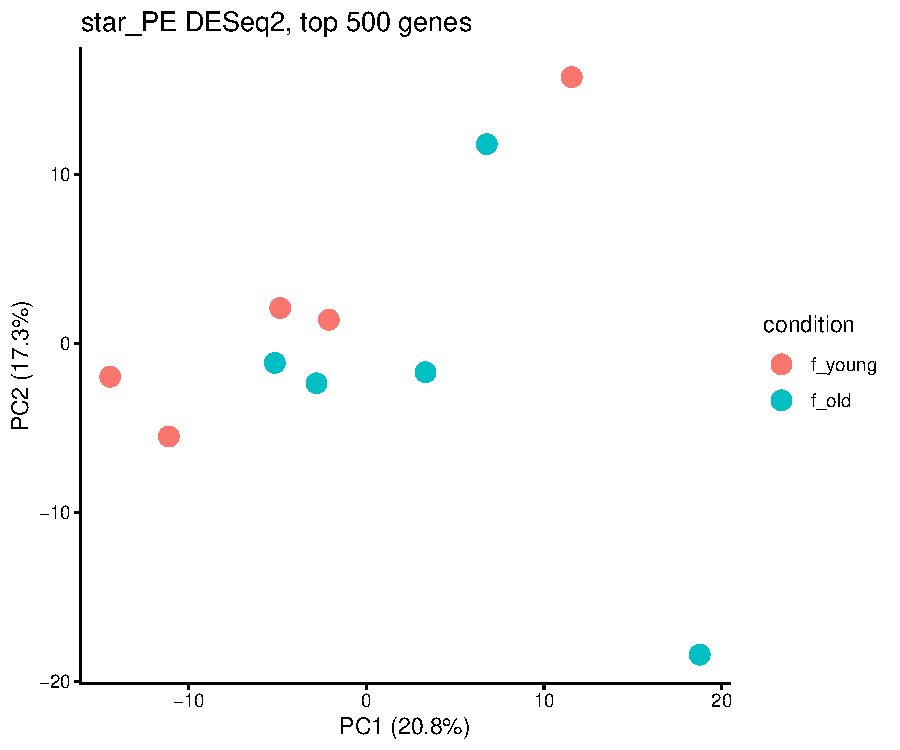
\includegraphics[width=0.4\linewidth,height=\textheight,keepaspectratio]{./results/plots/deseq2/pca/star_PE_pca_top500.pdf}

}

\caption{PCA de las muestras analizadas con DESeq2 y alineadas con STAR,
utilizando los 500 genes con mayor varianza. El análisis muestra una
tenue separación entre los grupos de edad, que puede sugerir la
presencia de cambios asociados al envejecimiento en corteza prefrontal
dorsolateral de \emph{Macaca mulatta} pero con un grado importante de
heterogeneidad biológica entre muestras.}

\end{figure}%

Se observa heterogeneidad en general entre los grupos de edades, por lo
que los PCs 1 y 2 no parecen explicar en gran medida la variabilidad de
la edad, sino un compilado de otros aspectos, sean técnicos o
biológicos. Dado que no se cuenta con metadatos adicionales para modelar
un factor de confusión que pudiera ocasionar variabilidad técnica,
aunado a que el envejecimiento cerebral es un proceso gradual {[}1{]},
se opta por continuar con los análisis \emph{downstream}.

\begin{figure}[H]

{\centering 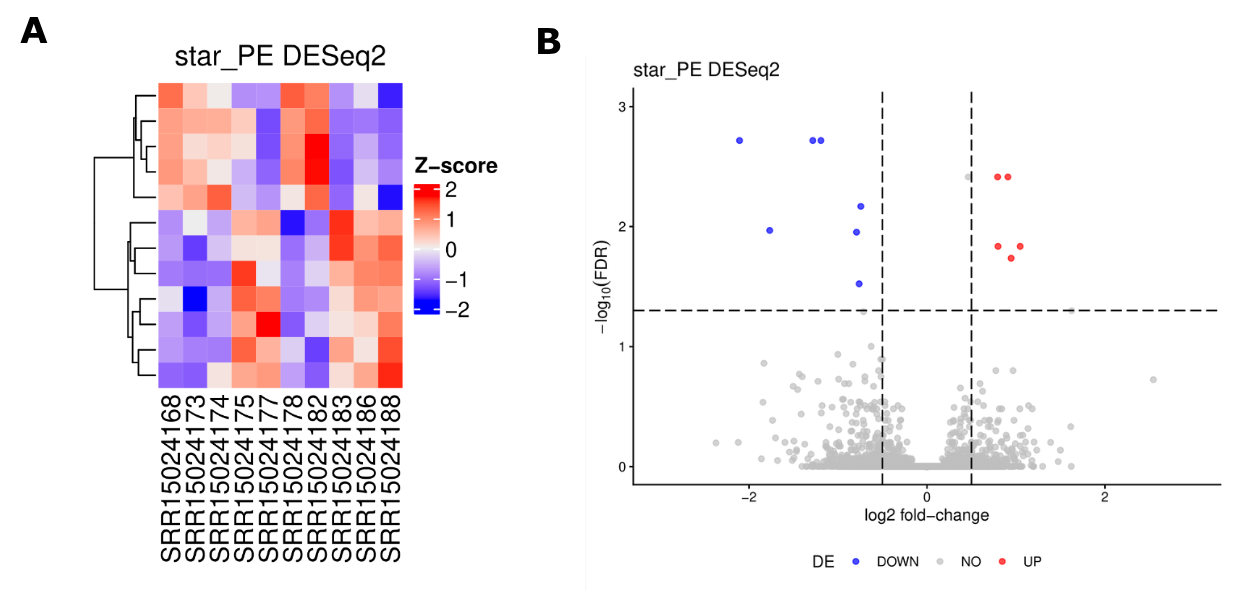
\includegraphics[width=0.6\linewidth,height=\textheight,keepaspectratio]{./results/plots/deseq2/de_deseq2_plots.png}

}

\caption{Gráficos de los resultados de DESeq2. A. Heatmap de los genes
diferencialmente expresados más significativos obtenidos con DESeq2 a
partir de alineamientos realizados con STAR. Se muestran los niveles de
expresión normalizados (TPM log2 transformados a Z-score por gen) para
las muestras jóvenes y adultas de \emph{Macaca mulatta}. El patrón
observado evidencia cambios transcriptómicos asociados al
envejecimiento, aunque con heterogeneidad considerable entre muestras
biológicas. B. Volcano plot de genes diferencialmente expresados
obtenidos con DESeq2 a partir de alineamientos realizados con STAR. Se
muestran los valores de log2 fold-change frente a −log10(FDR). Se
consideraron como diferencialmente expresados aquellos genes con
\textbar log2FC\textbar{} \textgreater{} 0.5 y FDR \textless{} 0.05. Los
genes sobreexpresados en muestras adultas se muestran en rojo y los
subexpresados en azul.}

\end{figure}%

Los resultados obtenidos muestran diferencias de expresión génica a lo
largo de las muestras jóvenes y adultas, aunque con una variabilidad
biológica considerable entre individuos. Aun así, los patrones
observados sugieren cambios transcriptómicos moderados asociados con
envejecimiento cerebral en dlPFC de \emph{Macaca mulatta}.

\subsection{Enriquecimiento funcional}\label{enriquecimiento-funcional}

GO permite interpretar listas de DEG en términos de \textbf{procesos
biológicos} (BP), \textbf{funciones moleculares} (MF) y
\textbf{componentes celulares} (CC), proporcionando un marco
estructurado y controlado para clasificar genes y sus productos en
categorías jerárquicas, facilitando así la identificación de patrones
funcionales subyacentes a los cambios de expresión observados. Así, se
realizaron análisis de enriquecimiento funcional basados en términos de
\textbf{GO} (\emph{Gene Ontology}) y \textbf{KEGG} con \textbf{DAVID},
la reconstrucción de las redes de interacción \emph{proteína-proteína}
mediante \textbf{STRING}, y \textbf{GSEA} (\emph{Gene Set Enrichment
Analysis}), a partir del \emph{ranking} global {[}15{]}.

Debido a que las colecciones funcionales de \textbf{MSigDB} {[}16{]} se
encuentran principalmente curadas para \emph{Homo sapiens} y no existen
colecciones \emph{Hallmark} específicas para \emph{Macaca mulatta}, los
DEG fueron convertidos a sus ortólogos humanos mediante la tabla de
correspondencia entre nombres y IDs y el paquete de \texttt{R}
\texttt{homologene} {[}17{]}, aprovechando la alta conservación
funcional entre primates. Se obtuvieron 10,956 ortólogos humanos,
guardados en \texttt{./results/GO/mmul\_human\_orthologs.tsv}, con los
identificadores originales de macaco y los símbolos asociados de ambas
especies. De la misma forma, todos los conjuntos de genes del análisis
de expresión diferencial (DEG, UP, DOWN y ALL) se exportan con los
nombres comunes ortólogos humanos, y se utiliza su taxonomía para los
análisis subsecuentes.

A pesar de haber obtenido 12 DEG (7 DOWN y 5 UP), se probó
\href{https://davidbioinformatics.nih.gov/workspace.html}{\texttt{DAVID}}
{[}18,19{]} con la intersección de cada lista con la tabla de homología,
de 3 genes cada una, de forma independiente. Los genes sobreexpresados
no arrojaron resultados significativos, mientras que los subexpresados
arrojaron 4 términos con un \emph{EASE threshold} de 0.1 y un
\emph{Count treshold} de 2, con \emph{Homo sapiens} como taxonomía, el
conjunto de genes presentes tras el filtrado de baja expresión como
\emph{background} y cargando únicamente la lista de los tres DEG
\emph{DOWN} (\texttt{./results/GO/DESeq2/star\_PE\_down.tsv}).

Si bien no se obtuvieron términos significativamente enriquecidos tras
corrección por múltiples pruebas, posiblemente debido a los pocos DEG
detectados, DAVID identificó funciones asociadas principalmente con
procesos apoptóticos e inmunológicos. En particular, los genes
\texttt{IFI27} y \texttt{TNFRSF1A} estuvieron asociados consistentemente
con términos relacionados con apoptosis y respuesta inmune, lo que
sugiere posibles cambios transcriptómicos vinculados con estrés celular
y neuroinflamación durante el envejecimiento cerebral. Posteriormente,
se probó \href{https://bioinformatics.sdstate.edu/go/}{\texttt{ShinyGO}}
{[}20{]} con la lista de todos los DEG en aras de comparar los
resultados pero no se obtuvieron enriquecimientos significativos.

\begin{table}[H]

\caption{\label{tbl-david-summarized}Tabla de términos enriquecidos en
DAVID para genes subexpresados con DESeq2 y STAR. Se incluyen las
columnas de categoría, término, p-value, Benjamini, fold enrichment y
genes asociados. Los términos se ordenan por p-value de forma
ascendente.}

\centering{

\begin{verbatim}
                   Category  ...                Genes
0  UP_KW_BIOLOGICAL_PROCESS  ...       IFI27,TNFRSF1A
1            UP_SEQ_FEATURE  ...  MC4R,IFI27,TNFRSF1A
2  UP_KW_BIOLOGICAL_PROCESS  ...       IFI27,TNFRSF1A
3          GOTERM_BP_DIRECT  ...       IFI27,TNFRSF1A

[4 rows x 6 columns]
\end{verbatim}

}

\end{table}%

Asimismo, \href{https://string-db.org}{\texttt{STRING}} (\emph{Search
Tool for the Retrieval of Interacting Genes/Proteins}) fue utilizado
para evaluar la existencia de módulos funcionales o redes regulatorias
entre los DEG, buscando asociaciones a procesos biológicos concretos
{[}21{]}. Para ello, se cargó la \textbf{lista completa de DEG},
igualmente con ortólogos humanos
(\texttt{./results/GO/DESeq2/star\_PE\_deg\_genes.tsv}), con \emph{Homo
Sapiens} como referencia. Se empleó la red completa de interacciones
provista por la plataforma, que toma en cuenta asociaciones derivadas de
evidencia experimental, bases de datos, coexpresión y minería de
literatura {[}21{]}, con un umbral de confianza medio (\emph{medium
confidence}, 0.4).

\begin{figure}[H]

{\centering 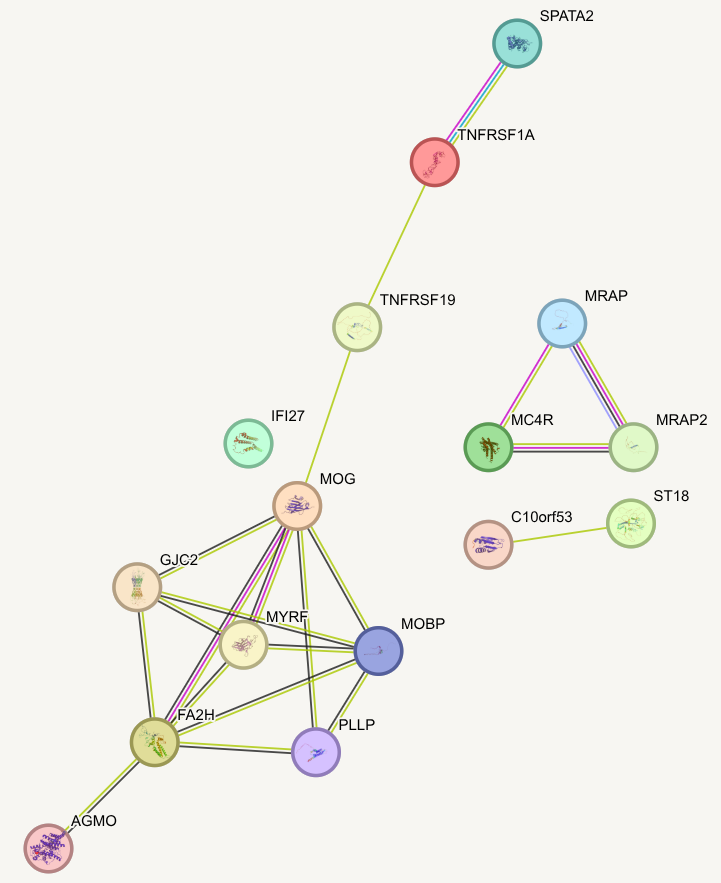
\includegraphics[width=0.4\linewidth,height=\textheight,keepaspectratio]{./results/GO/DESeq2/STRING/1_string_network.png}

}

\caption{Red de interacción proteína--proteína generada en STRING,
utilizando los genes diferencialmente expresados obtenidos mediante
DESeq2. Se observaron agrupamientos funcionales asociados principalmente
con procesos de mielinización y oligodendrocitos, destacando genes como
MOG, MOBP, PLLP y FA2H. También se identificó un pequeño módulo
relacionado con inflamación y apoptosis, incluyendo TNFRSF1A y SPATA2.
Las conexiones representan asociaciones funcionales conocidas o
predichas entre proteínas.}

\end{figure}%

\begin{figure}[H]

{\centering 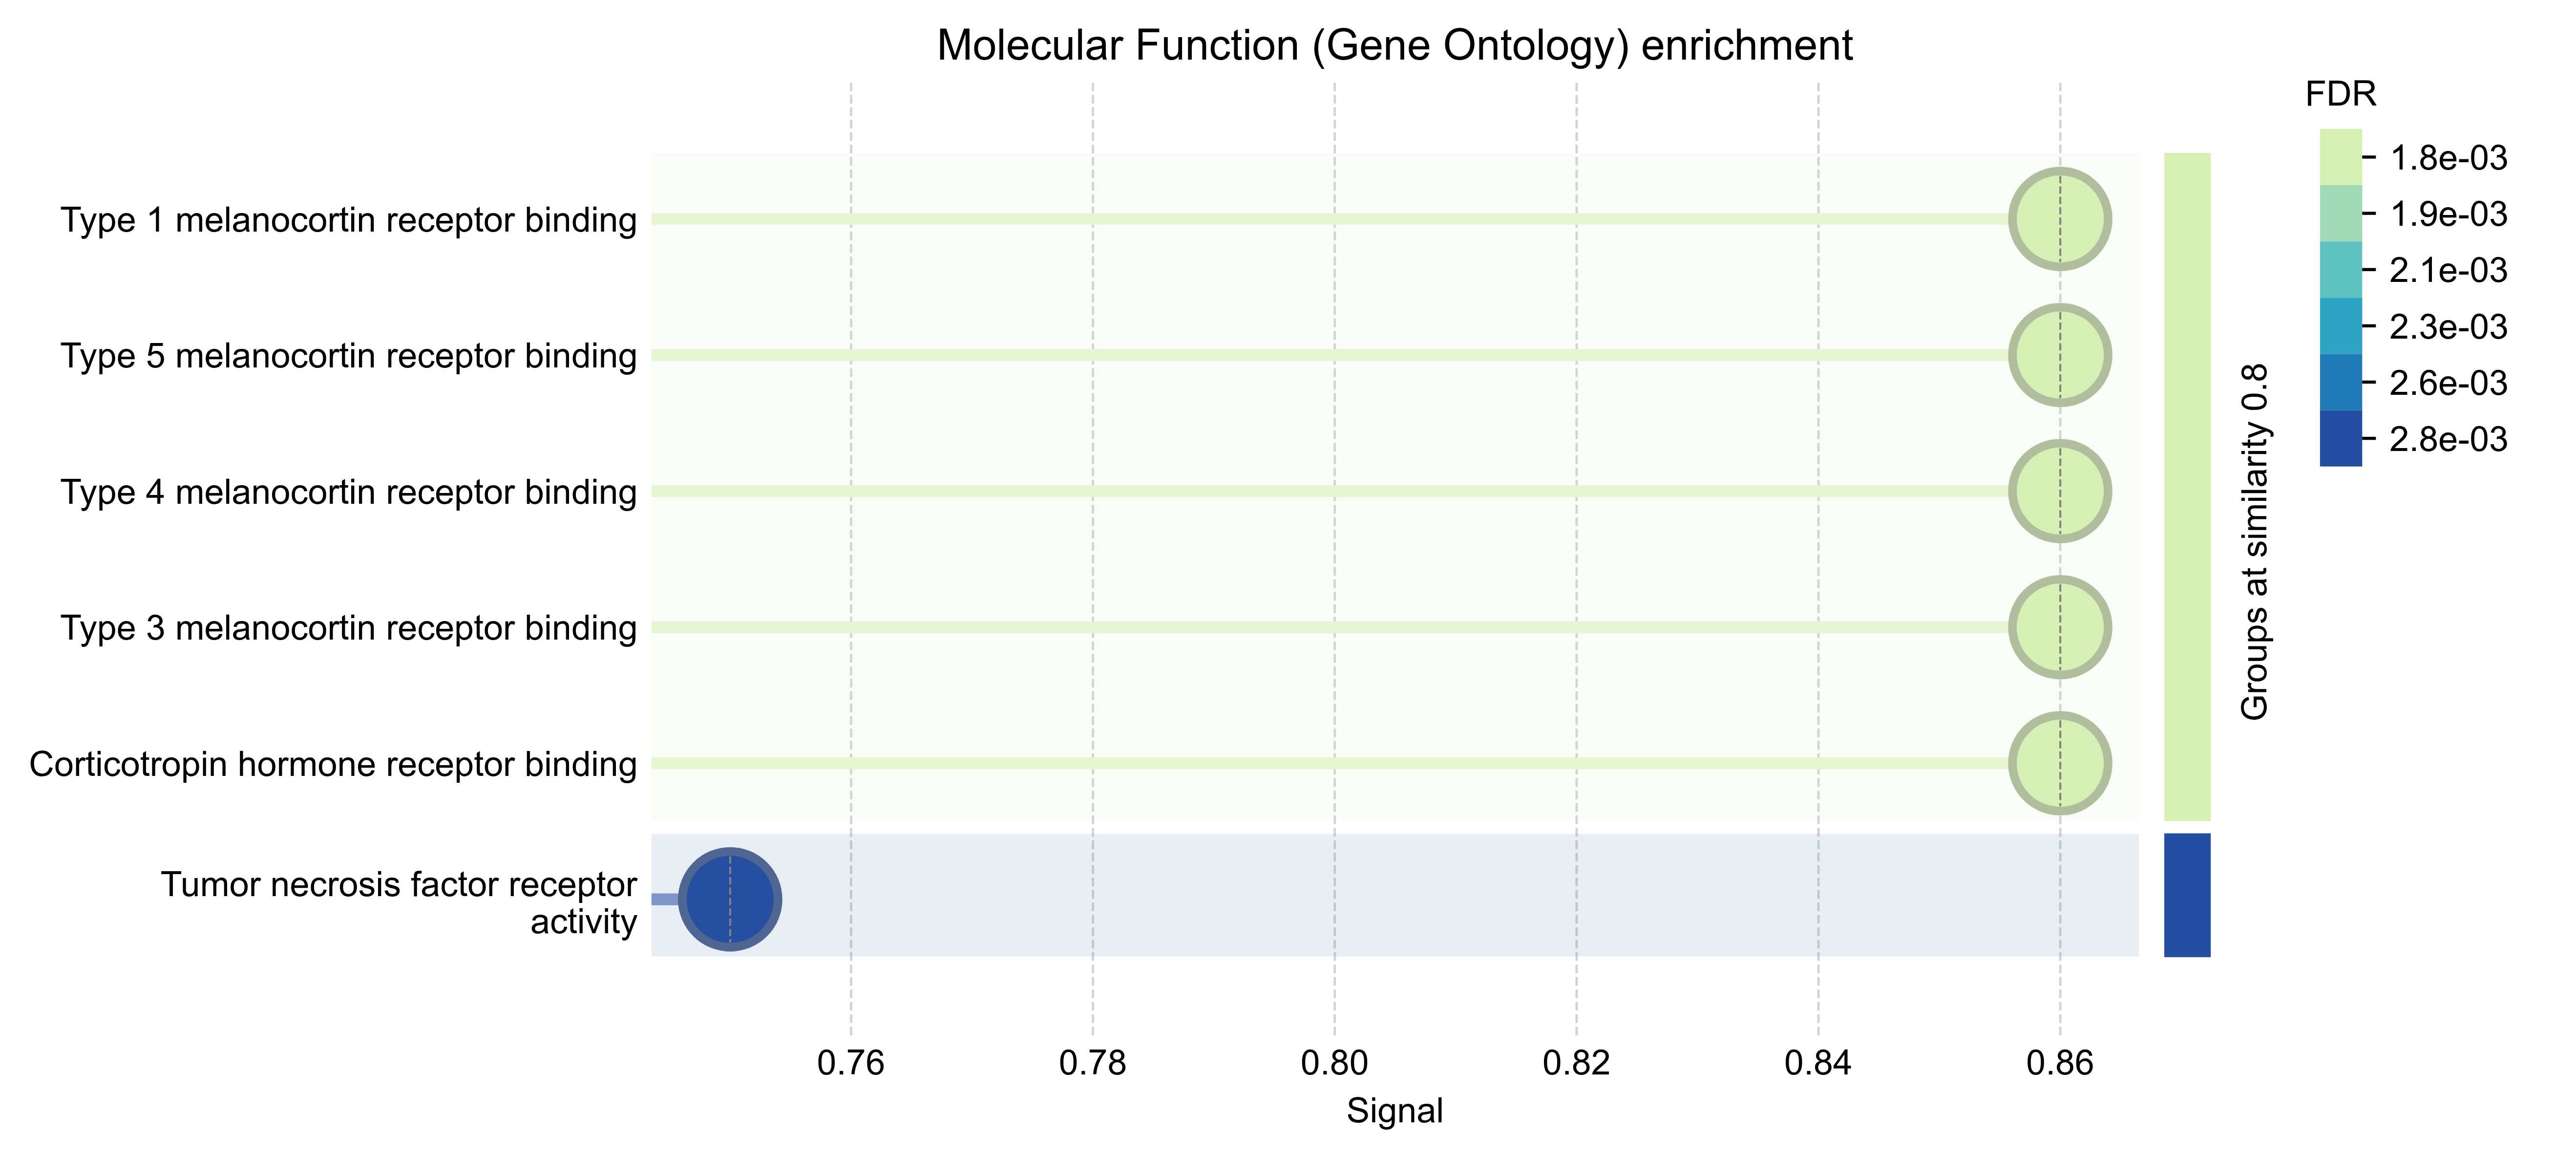
\includegraphics[width=1\linewidth,height=\textheight,keepaspectratio]{./results/GO/DESeq2/STRING/2_string_enrichment_plot.png}

}

\caption{Gráfico de enriquecimiento funcional generado en STRING basado
en anotaciones funcionales y publicaciones asociadas. Los términos
enriquecidos mostraron asociaciones en mayor medida con receptores
melanocortínicos y actividad relacionada con receptores de TNF. El
tamaño de los puntos representa la magnitud de la señal de
enriquecimiento y el color corresponde a la tasa de descubrimiento falso
(FDR).}

\end{figure}%

La red resultante mostró agrupamientos funcionales coherentes, como un
conjunto de genes relacionados con \textbf{mielina} y
\textbf{oligodendrocitos}, que podrían implicar alteraciones sutiles
asociadas en estas durante el envejecimiento. Adicionalmente, algunos
genes se asociaron con procesos inflamatorios y apoptóticos. Asimismo,
los términos enriquecidos obtenidos se relacionaron con señalización
mediada por receptores melanocortínicos y funciones inmunes asociadas a
receptores de TNF. Pese al número de genes diferencialmente expresados,
ambos análisis mostraron consistencia entre sí mismos.

Dado que la cantidad de genes diferencialmente expresados en general era
limitada, se realizó un análisis de \textbf{GSEA} (\emph{Gene Set
Enrichment Analysis}) con el ranking global de genes ordenados por la
columna \texttt{res} de \texttt{DESeq2}, derivado del \emph{estadístico
de Wald}, que recapitula sobre la dirección y magnitud de expresión de
los genes {[}22{]}. El análisis se llevó a cabo en modo
\emph{preranked}, utilizando las colecciones de conjuntos de genes
\emph{Hallmark} de \textbf{MSigDB} de \emph{homo sapiens} {[}16{]} y
haciendo 1,000 permutaciones con conjuntos de entre 15 y 500 genes.

\begin{figure}[H]

{\centering 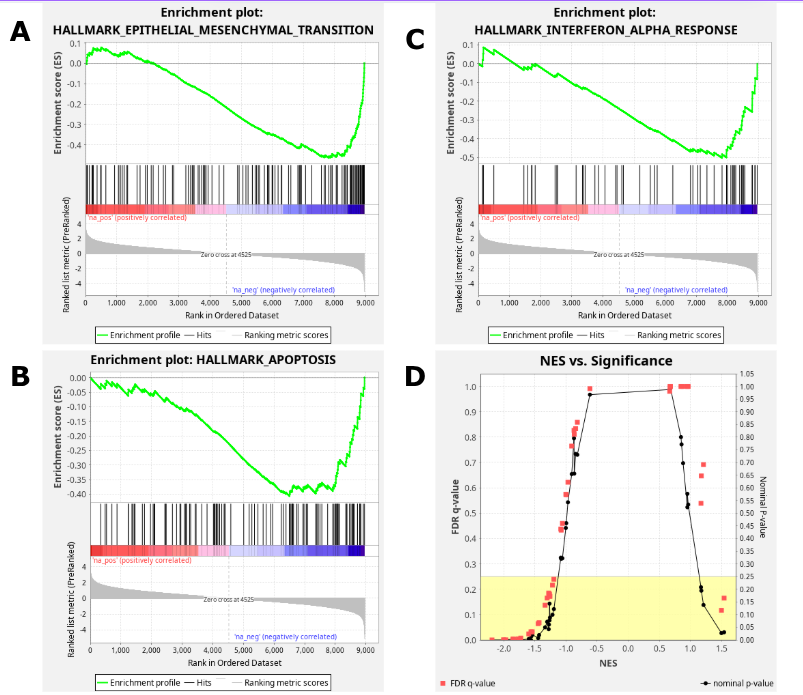
\includegraphics[width=0.85\linewidth,height=\textheight,keepaspectratio]{results/plots/gsea/3_gsea_hallmarks.png}

}

\caption{Resultados representativos del análisis GSEA utilizando
colecciones Hallmark de MSigDB. A. Enriquecimiento negativo del conjunto
HALLMARK\_EPITHELIAL\_MESENCHYMAL\_TRANSITION, indicando una acumulación
coordinada de genes asociados a remodelación tisular hacia el extremo
correspondiente a las muestras jóvenes. B. Enriquecimiento negativo del
conjunto HALLMARK\_APOPTOSIS, sugiriendo una mayor representación
relativa de genes relacionados con apoptosis y respuesta a estrés
celular en muestras jóvenes. C. Enriquecimiento negativo del conjunto
HALLMARK\_INTERFERON\_ALPHA\_RESPONSE, consistente con activación
coordinada de genes asociados a señalización inmune e interferón. D.
Relación entre el normalized enrichment score (NES) y la significancia
estadística de los conjuntos Hallmark evaluados. Los puntos resaltados
corresponden a conjuntos significativamente enriquecidos.}

\end{figure}%

\begin{figure}[H]

{\centering 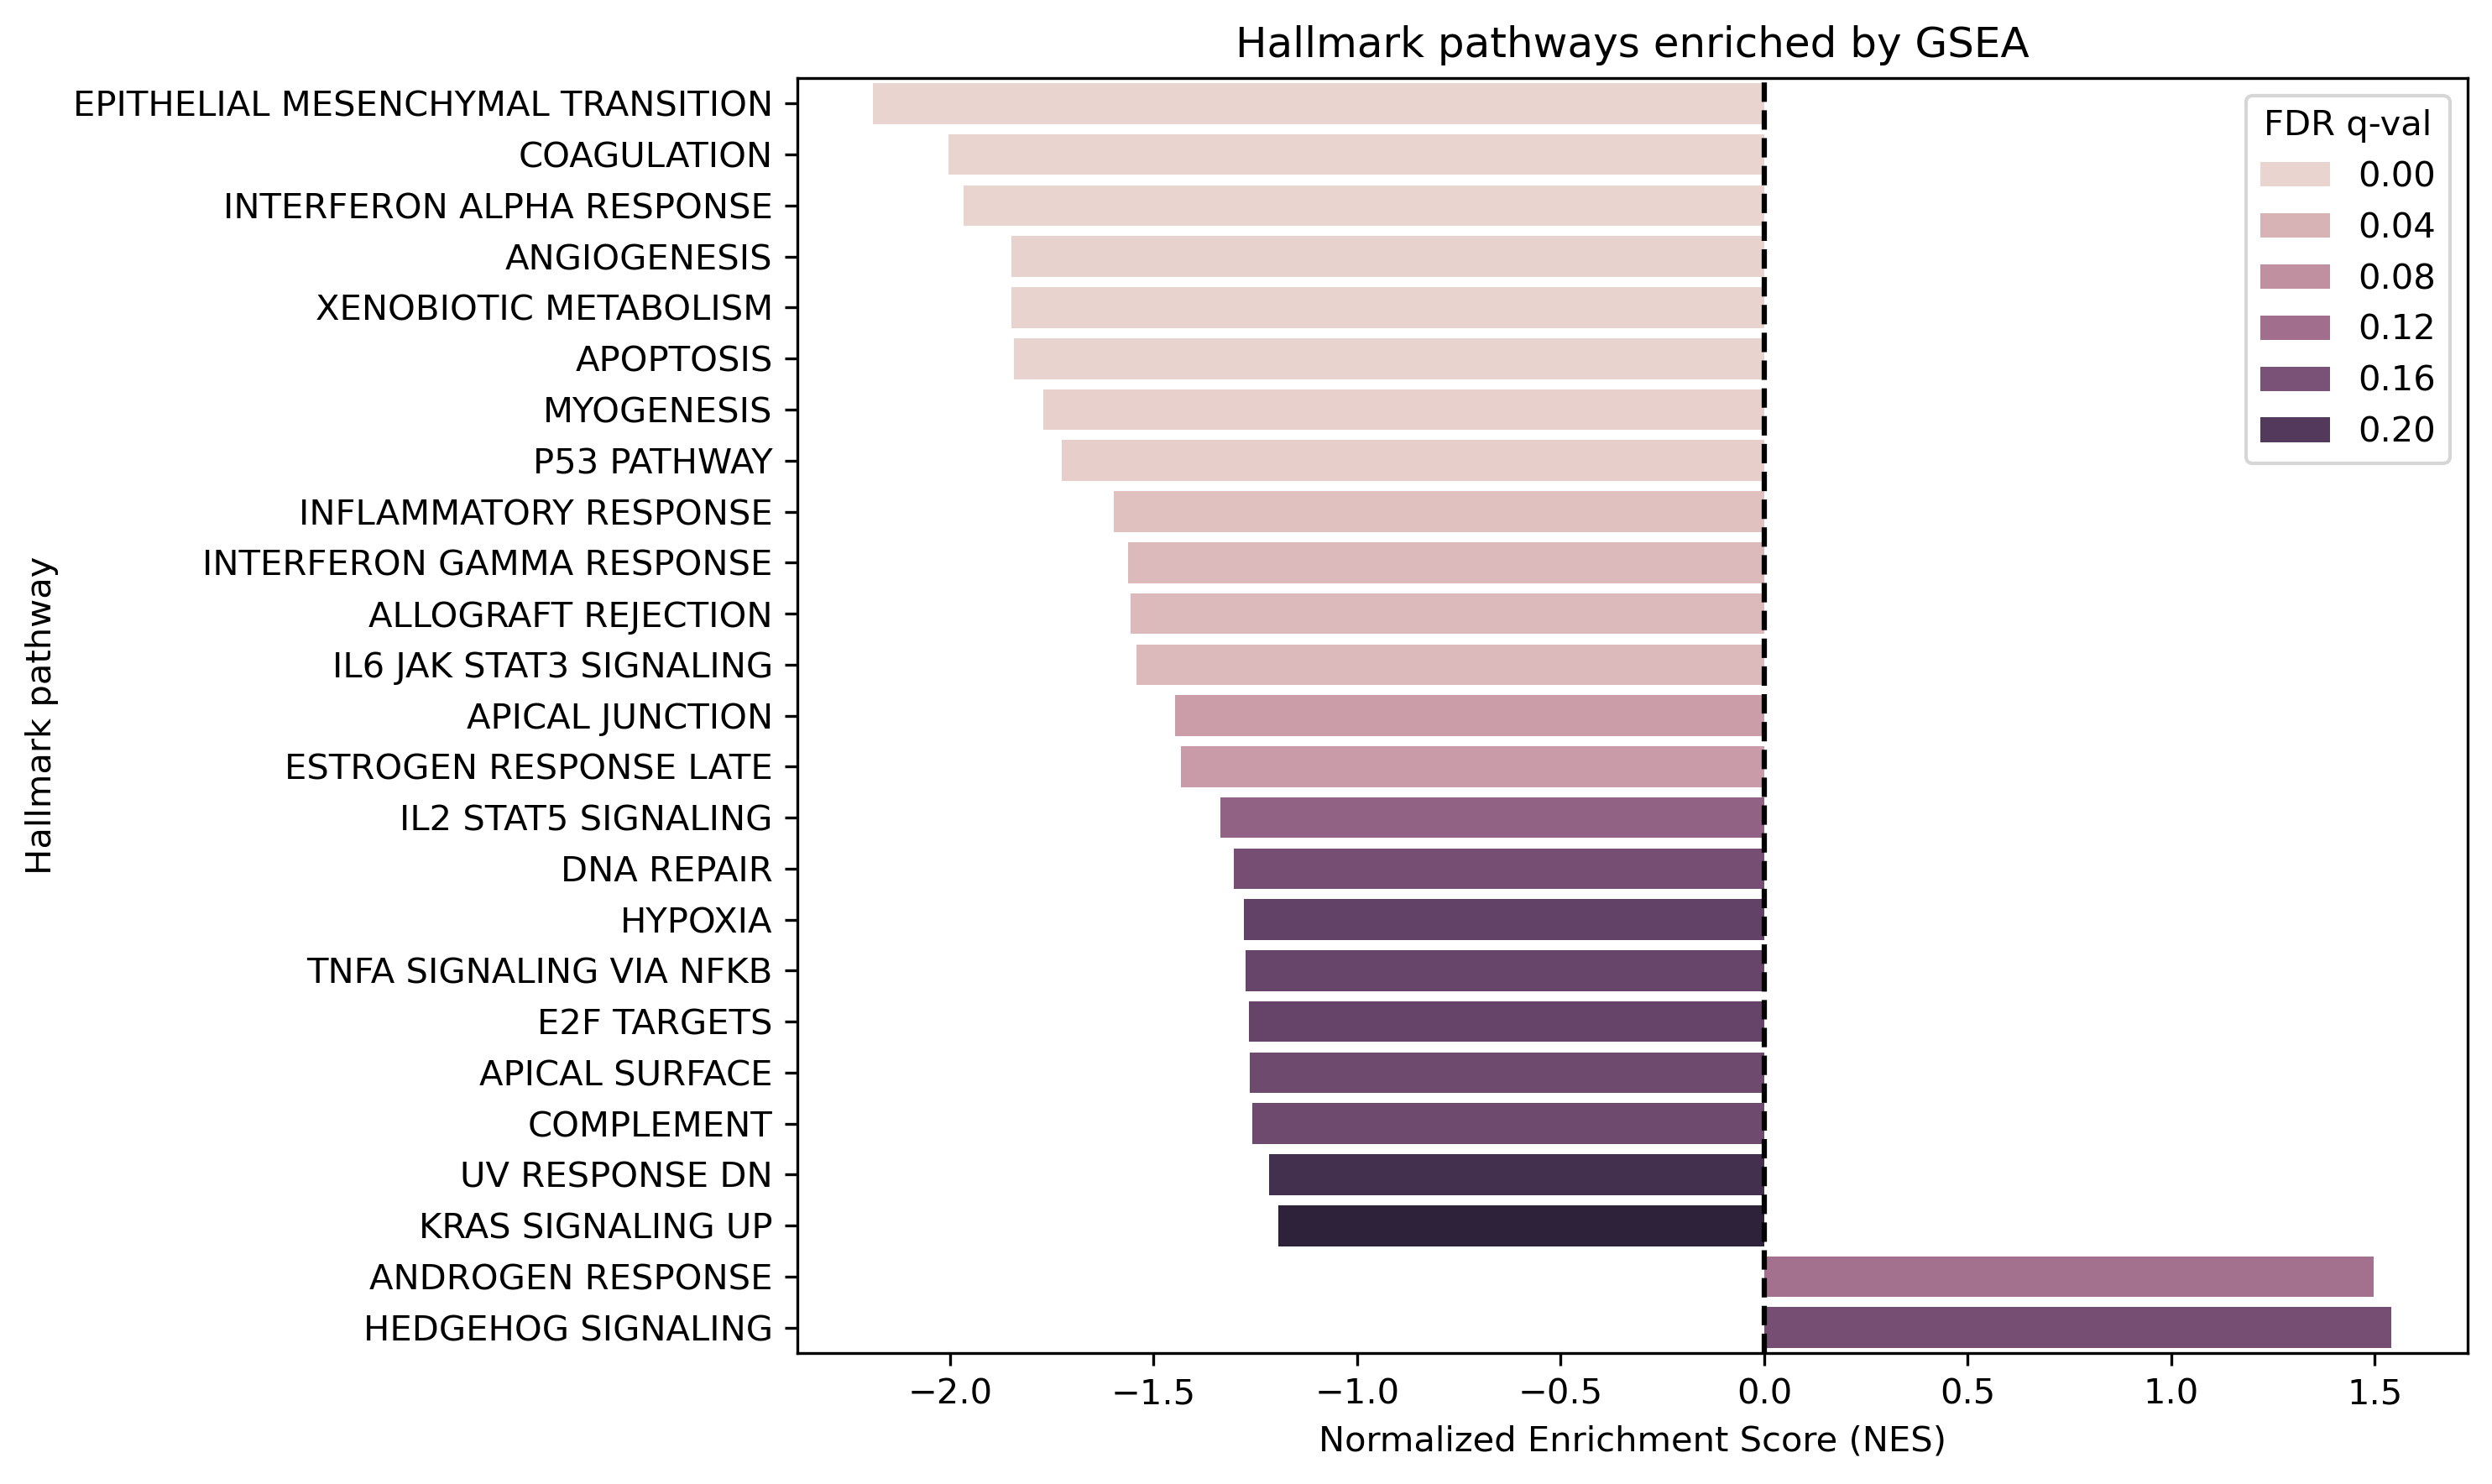
\includegraphics[width=0.9\linewidth,height=\textheight,keepaspectratio]{./results/plots/gsea/gsea_hallmark_barplot.png}

}

\caption{Resumen global de los resultados de GSEA para colecciones
Hallmark. El eje X muestra el normalized enrichment score (NES) de cada
conjunto génico y el eje Y los procesos biológicos evaluados. Los
valores negativos indican enriquecimiento relativo hacia genes más
altamente expresados en muestras jóvenes, mientras que los valores
positivos indican enriquecimiento hacia muestras viejas. Los colores
representan la significancia estadística corregida por FDR. Destacan
procesos relacionados con transición epitelio-mesénquima, respuesta
inflamatoria, señalización por interferón, apoptosis y angiogénesis.}

\end{figure}%

Se obtuvo un enriquecimiento significativo de vías relacionadas con
respuesta inflamatoria, señalización por interferón, apoptosis,
angiogénesis y transición epitelio-mesénquima (EMT). En general, estos
conjuntos presentaron valores negativos de NES, indicador de un mayor
representación relativa hacia genes más expresados en muestras jóvenes.

\section{Discusión}\label{discusiuxf3n}

El análisis realizado posibilitó la identificación de cambios de
expresión génica asociados con envejecimiento cerebral en corteza
prefrontal dorsolateral de \emph{Macaca mulatta}. Aunque el número de
genes diferencialmente expresados fue relativamente reducido bajo los
criterios de significancia empleados, los resultados obtenidos con
análisis sobre el \emph{ranking} global muestran tendencias
biológicamente consistentes con procesos reportados previamente durante
envejecimiento cerebral normal.

Los genes diferencialmente expresados y los análisis de enriquecimiento
sugieren alteraciones relacionadas con señalización neuronal, respuesta
al estrés y procesos inmunológicos. En particular, los análisis
funcionales apuntan hacia una disminución de procesos asociados con
actividad sináptica y regulación neuronal, así como cambios en rutas
relacionadas con inflamación y respuesta celular. Estos resultados son
congruentes con observaciones reportadas en el artículo original
{[}1{]}, donde el envejecimiento cerebral en macacos se asoció con
disminución de genes relacionados con función neuronal y aumento de
procesos asociados con respuesta inmune e inflamación.

El agrupamiento observado en el \emph{heatmap} sugiere, además, la
existencia de perfiles transcriptómicos parcialmente diferenciados entre
muestras jóvenes y adultas. Esto indica que, aún con un tamaño de
muestra limitado, es posible recuperar señales biológicas asociadas con
la edad. De forma similar, el análisis de GSEA mostró enriquecimiento de
conjuntos génicos relacionados con envejecimiento, metabolismo y
respuesta celular, reforzando la consistencia biológica de los
resultados obtenidos.

Inevitablemente, este trabajo presenta varias limitaciones. En primer
lugar, el tamaño de muestra fue reducido, lo que disminuye la potencia
estadística y probablemente limita la detección de DEG. Asimismo, el
análisis se restringió a hembras y a una única región cerebral, por lo
que los resultados no necesariamente representan procesos globales de
envejecimiento cerebral. Aunado, al tratarse de datos de \emph{bulk}
RNA-seq, los cambios observados reflejan señales promedio de múltiples
tipos celulares y no permiten distinguir contribuciones específicas de
poblaciones neuronales o gliales concretas.

A pesar de estas limitaciones, el pipeline implementado permitió
reproducir múltiples tendencias biológicas descritas previamente para
envejecimiento cerebral en primates, mostrando que los análisis de
RNA-seq constituyen una herramienta útil para estudiar procesos
moleculares complejos asociados con envejecimiento y neurobiología,
junto con la importancia de considerar la heterogeneidad biológica y las
limitaciones inherentes a los propios datos disponibles al interpretar
los resultados. Más aún, a esto le subyace la necesidad de la correcta
selección de datos al llevar a cabo análisis que precisen de
significancia estadística y, sobre todo, el sesgo de estudios que existe
hacia organismos modelo más estudiados, lo que limita la disponibilidad
de datos y herramientas para estudiar procesos biológicos en especies no
tan comunes y dificulta, por tanto, los hallazgos de procesos
moleculares con implicaciones clínicas potenciales.

\section{Conclusiones}\label{conclusiones}

Los resultados obtenidos permitieron identificar cambios
transcriptómicos asociados con envejecimiento cerebral en corteza
prefrontal dorsolateral, particularmente en procesos relacionados con
señalización neuronal, respuesta inmune y estrés celular. Aunque el
número de genes diferencialmente expresados fue limitado, los patrones
observados fueron consistentes entre sí mismos y con hallazgos
reportados previamente en estudios de envejecimiento cerebral en
primates.

El uso de herramientas como \texttt{DESeq2}, \texttt{GSEA} y análisis de
enriquecimiento funcional permitió interpretar los cambios de expresión
génica dentro de un contexto biológico amplio, resaltando la utilidad de
los enfoques transcriptómicos para estudiar mecanismos moleculares
asociados con envejecimiento cerebral y demostrando que el análisis
bioinformático de datos de RNA-seq permite recuperar señales
biológicamente relevantes incluso a partir de subconjuntos reducidos y
heterogéneos de muestras. Así, si bien constituye una aproximación útil
para explorar procesos de envejecimiento y regulación génica en sistemas
complejos, exhibe las limitaciones de estos estudios cuando se cuenta
con un número reducido de muestras, los patrones de expresión no son tan
pronunciados, se carece de un universo extenso de metadatos para modelar
factores de confusión o se trabaja con especies especies no modelo con
anotaciones menos completas.

\newpage

\section{Referencias}\label{referencias}

\phantomsection\label{refs}
\begin{CSLReferences}{0}{1}
\bibitem[\citeproctext]{ref-chiou-2022}
\CSLLeftMargin{1. }%
\CSLRightInline{Kenneth L. Chiou, Alex R. DeCasien, Katherina P. Rees,
Camille Testard, Cailyn H. Spurrell, Aishwarya A. Gogate, Hannah A.
Pliner, Sébastien Tremblay, Arianne Mercer, Connor J. Whalen, Josué E.
Negrón-Del Valle, Mareike C. Janiak, Samuel E. Bauman Surratt, Olga
González, Nicole R. Compo, Michala K. Stock, Angelina V. Ruiz-Lambides,
Melween I. Martínez, Melissa A. Wilson, Amanda D. Melin, Susan C. Antón,
Christopher S. Walker, Jérôme Sallet, Jason M. Newbern, Lea M. Starita,
Jay Shendure, James P. Higham, Lauren J. N. Brent, Michael J. Montague,
Michael L. Platt, Noah Snyder-Mackler. {Multiregion transcriptomic
profiling of the primate brain reveals signatures of aging and the
social environment}. Nature Neuroscience. 2022 Nov;25(12):1714--23.
doi:\href{https://doi.org/10.1038/s41593-022-01197-0}{10.1038/s41593-022-01197-0}}

\bibitem[\citeproctext]{ref-sratoolkit}
\CSLLeftMargin{2. }%
\CSLRightInline{NCBI Sequence Read Archive. SRA toolkit {[}Internet{]}.
2026. Available from: \url{https://github.com/ncbi/sra-tools}}

\bibitem[\citeproctext]{ref-FastQC}
\CSLLeftMargin{3. }%
\CSLRightInline{Simon Andrews. FastQC: A quality control tool for high
throughput sequence data {[}Internet{]}. 2010. Available from:
\url{https://www.bioinformatics.babraham.ac.uk/projects/fastqc/}}

\bibitem[\citeproctext]{ref-ewels-2016}
\CSLLeftMargin{4. }%
\CSLRightInline{Philip Ewels, Måns Magnusson, Sverker Lundin, Max
Käller. {MultiQC: summarize analysis results for multiple tools and
samples in a single report}. Bioinformatics. 2016 Jun;32(19):3047--8.
doi:\href{https://doi.org/10.1093/bioinformatics/btw354}{10.1093/bioinformatics/btw354}}

\bibitem[\citeproctext]{ref-vallegarcia2026curso}
\CSLLeftMargin{5. }%
\CSLRightInline{Ricardo Valle García. Curso de transcript{ó}mica 2026:
Anotaci{ó}n funcional y enriquecimiento biol{ó}gico. 2026.}

\bibitem[\citeproctext]{ref-chen-2018}
\CSLLeftMargin{6. }%
\CSLRightInline{Shifu Chen, Yanqing Zhou, Yaru Chen, Jia Gu. {fastp: an
ultra-fast all-in-one FASTQ preprocessor}. Bioinformatics. 2018
Jul;34(17):i884--90.
doi:\href{https://doi.org/10.1093/bioinformatics/bty560}{10.1093/bioinformatics/bty560}}

\bibitem[\citeproctext]{ref-dobin2013star}
\CSLLeftMargin{7. }%
\CSLRightInline{Alexander Dobin, Carrie A. Davis, Felix Schlesinger,
Jorg Drenkow, Chris Zaleski, Sonali Jha, Philippe Batut, Mark Chaisson,
Thomas R. Gingeras. STAR: Ultrafast universal RNA-seq aligner.
Bioinformatics. 2013;29(1):15--21.
doi:\href{https://doi.org/10.1093/bioinformatics/bts635}{10.1093/bioinformatics/bts635}}

\bibitem[\citeproctext]{ref-kim2019hisat2}
\CSLLeftMargin{8. }%
\CSLRightInline{Daehwan Kim, Joseph M. Paggi, Chanhee Park, Christopher
Bennett, Steven L. Salzberg. Graph-based genome alignment and genotyping
with HISAT2 and HISAT-genotype. Nature Biotechnology.
2019;37(8):907--15.
doi:\href{https://doi.org/10.1038/s41587-019-0201-4}{10.1038/s41587-019-0201-4}}

\bibitem[\citeproctext]{ref-Ensembl2025}
\CSLLeftMargin{9. }%
\CSLRightInline{Andrew D. Yates, others. Ensembl 2025. Nucleic Acids
Research. 2025;53(D1):DXXX--.
doi:\href{https://doi.org/10.1093/nar/gkae1071}{10.1093/nar/gkae1071}}

\bibitem[\citeproctext]{ref-li-2009}
\CSLLeftMargin{10. }%
\CSLRightInline{Heng Li, Bob Handsaker, Alec Wysoker, Tim Fennell, Jue
Ruan, Nils Homer, Gabor Marth, Goncalo Abecasis, Richard Durbin, Genome
Project Data Processing Subgroup. {The Sequence Alignment/Map format and
SAMtools}. Bioinformatics. 2009 Jun;25(16):2078--9.
doi:\href{https://doi.org/10.1093/bioinformatics/btp352}{10.1093/bioinformatics/btp352}}

\bibitem[\citeproctext]{ref-liao-2013}
\CSLLeftMargin{11. }%
\CSLRightInline{Yang Liao, Gordon K. Smyth, Wei Shi. {featureCounts: an
efficient general purpose program for assigning sequence reads to
genomic features}. Bioinformatics. 2013 Nov;30(7):923--30.
doi:\href{https://doi.org/10.1093/bioinformatics/btt656}{10.1093/bioinformatics/btt656}}

\bibitem[\citeproctext]{ref-love2014deseq2}
\CSLLeftMargin{12. }%
\CSLRightInline{Michael I. Love, Wolfgang Huber, Simon Anders. Moderated
estimation of fold change and dispersion for RNA-seq data with DESeq2.
Genome Biology. 2014;15(12):550.
doi:\href{https://doi.org/10.1186/s13059-014-0550-8}{10.1186/s13059-014-0550-8}}

\bibitem[\citeproctext]{ref-robinson2010edger}
\CSLLeftMargin{13. }%
\CSLRightInline{Mark D. Robinson, Davis J. McCarthy, Gordon K. Smyth.
edgeR: A bioconductor package for differential expression analysis of
digital gene expression data. Bioinformatics. 2010;26(1):139--40.
doi:\href{https://doi.org/10.1093/bioinformatics/btp616}{10.1093/bioinformatics/btp616}}

\bibitem[\citeproctext]{ref-vallegarcia2026deseq2}
\CSLLeftMargin{14. }%
\CSLRightInline{David Valle-Garcia. Clase 8 - análisis de expresión
diferencial con DESeq2. Material de curso en HTML generado con Quarto;
2026.}

\bibitem[\citeproctext]{ref-vallegarcia2026anotaciones}
\CSLLeftMargin{15. }%
\CSLRightInline{Ricardo Valle García. Notas de anotaci{ó}n funcional
para RNA-seq. 2026.}

\bibitem[\citeproctext]{ref-liberzon-2015}
\CSLLeftMargin{16. }%
\CSLRightInline{Arthur Liberzon, Chet Birger, Helga Thorvaldsdóttir,
Mahmoud Ghandi, Jill P. Mesirov, Pablo Tamayo. {The Molecular Signatures
Database Hallmark Gene Set Collection}. Cell Systems. 2015
Dec;1(6):417--25.
doi:\href{https://doi.org/10.1016/j.cels.2015.12.004}{10.1016/j.cels.2015.12.004}}

\bibitem[\citeproctext]{ref-mancarci-2018}
\CSLLeftMargin{17. }%
\CSLRightInline{Ogan Mancarci. {homologene: Quick Access to Homologene
and Gene Annotation Updates} {[}Internet{]}. 2018. Available from:
\url{https://doi.org/10.32614/cran.package.homologene}
doi:\href{https://doi.org/10.32614/cran.package.homologene}{10.32614/cran.package.homologene}}

\bibitem[\citeproctext]{ref-huang2008}
\CSLLeftMargin{18. }%
\CSLRightInline{Da Wei Huang, Brad T. Sherman, Richard A. Lempicki.
Systematic and integrative analysis of large gene lists using DAVID
bioinformatics resources. Nature Protocols. 2009;4(1):44--57.
doi:\href{https://doi.org/10.1038/nprot.2008.211}{10.1038/nprot.2008.211}}

\bibitem[\citeproctext]{ref-sherman2022}
\CSLLeftMargin{19. }%
\CSLRightInline{Brad T. Sherman, Ming Hao, Jiao Qiu, Xiaoli Jiao,
Michael W. Baseler, H. Clifford Lane, Tomozumi Imamichi, Wenyi Chang.
DAVID: A web server for functional enrichment analysis and functional
annotation of gene lists (2021 update). Nucleic Acids Research.
2022;50(W1):W216--21.
doi:\href{https://doi.org/10.1093/nar/gkac194}{10.1093/nar/gkac194}}

\bibitem[\citeproctext]{ref-ge-2019}
\CSLLeftMargin{20. }%
\CSLRightInline{Steven Xijin Ge, Dongmin Jung, Runan Yao. {ShinyGO: a
graphical gene-set enrichment tool for animals and plants}.
Bioinformatics. 2019 Dec;36(8):2628--9.
doi:\href{https://doi.org/10.1093/bioinformatics/btz931}{10.1093/bioinformatics/btz931}}

\bibitem[\citeproctext]{ref-szklarczyk2023string}
\CSLLeftMargin{21. }%
\CSLRightInline{Damian Szklarczyk, Rebecca Kirsch, Mikaela Koutrouli,
Katerina Nastou, Farrokh Mehryary, Radja Hachilif, Annika L. Gable, Tao
Fang, Nadezhda T. Doncheva, Sampo Pyysalo, others. The STRING database
in 2023: Protein--protein association networks and functional enrichment
analyses for any sequenced genome of interest. Nucleic Acids Research.
2023;51(D1):D638--46.
doi:\href{https://doi.org/10.1093/nar/gkac1000}{10.1093/nar/gkac1000}}

\bibitem[\citeproctext]{ref-subramanian2005}
\CSLLeftMargin{22. }%
\CSLRightInline{Aravind Subramanian, Pablo Tamayo, Vamsi K. Mootha,
Sayan Mukherjee, Benjamin L. Ebert, Michael A. Gillette, Amanda
Paulovich, Scott L. Pomeroy, Todd R. Golub, Eric S. Lander, Jill P.
Mesirov. Gene set enrichment analysis: A knowledge-based approach for
interpreting genome-wide expression profiles. Proceedings of the
National Academy of Sciences. 2005;102(43):15545--50.
doi:\href{https://doi.org/10.1073/pnas.0506580102}{10.1073/pnas.0506580102}}

\bibitem[\citeproctext]{ref-patro2017salmon}
\CSLLeftMargin{23. }%
\CSLRightInline{Rob Patro, Geet Duggal, Michael I. Love, Rafael A.
Irizarry, Carl Kingsford. Salmon provides fast and bias-aware
quantification of transcript expression. Nature Methods.
2017;14(4):417--9.
doi:\href{https://doi.org/10.1038/nmeth.4197}{10.1038/nmeth.4197}}

\bibitem[\citeproctext]{ref-rueda2015edger}
\CSLLeftMargin{24. }%
\CSLRightInline{Oscar Rueda, Bernard Pereira. Differential expression
analysis using edgeR. University of Cambridge; 2015.}

\end{CSLReferences}

\newpage

\section{Reproducibilidad}\label{reproducibilidad}

\subsection{Entorno de ejecución}\label{entorno-de-ejecuciuxf3n}

\begin{itemize}
\tightlist
\item
  Sistema operativo local: Linux Arch (\texttt{6.19.8-arch1-1})
\item
  Shell utilizada: \texttt{zsh\ 5.9}
\item
  Servidor de cómputo: \texttt{chaac}
\item
  Gestor de ambientes: \texttt{conda\ 2.5.0}
\item
  Documento generado mediante Quarto \texttt{1.8.27} con salida PDF vía
  LaTeX
\end{itemize}

\subsection{Versiones de software}\label{versiones-de-software}

\begin{itemize}
\tightlist
\item
  Python \texttt{3.11.14}
\item
  R \texttt{4.5.3}
\item
  FastQC \texttt{0.12.1}
\item
  MultiQC \texttt{1.33}
\item
  fastp \texttt{0.24.1}
\item
  STAR \texttt{2.7.11b}
\item
  HISAT2 \texttt{2.2.1}
\item
  samtools \texttt{1.21}
\item
  featureCounts/Subread \texttt{2.0.8}
\end{itemize}

\subsection{Datos utilizados}\label{datos-utilizados}

\begin{itemize}
\tightlist
\item
  Bioproyecto: \texttt{PRJNA743289}
\item
  GEO: \texttt{GSE179330}
\item
  Organismo: \emph{Macaca mulatta}
\item
  Genoma de referencia: \texttt{Mmul\_10}
\item
  Anotación génica: Ensembl Release 115
\end{itemize}

\subsection{Organización del
proyecto}\label{organizaciuxf3n-del-proyecto}

\begin{itemize}
\tightlist
\item
  \texttt{./data/}: datos crudos, referencias y archivos FASTQ
  procesados
\item
  \texttt{./scripts/}: automatización y scripts auxiliares
\item
  \texttt{./results/}: alineamientos, matrices de conteos, análisis
  diferenciales y enriquecimiento funcional
\item
  \texttt{./docs/}: portada, bibliografía y archivos auxiliares de
  renderizado
\end{itemize}

\subsection{Pipeline general}\label{pipeline-general}

\begin{enumerate}
\def\labelenumi{\arabic{enumi}.}
\tightlist
\item
  Descarga de datos mediante \texttt{fasterq-dump}
\item
  Control de calidad con FastQC y MultiQC
\item
  Limpieza y filtrado de lecturas con fastp
\item
  Alineamiento contra el genoma de referencia mediante STAR y HISAT2
\item
  Filtrado, ordenamiento e indexado de BAMs utilizando samtools
\item
  Cuantificación de abundancias génicas mediante featureCounts
\item
  Análisis de expresión diferencial con DESeq2
\item
  Análisis funcional mediante GO, STRING y GSEA
\end{enumerate}

\begin{quote}
Adicionalmente, los parámetros relevantes utilizados durante el análisis
fueron especificados explícitamente dentro del documento para facilitar
la reproducibilidad completa del pipeline.
\end{quote}

\newpage

\section{Anexo}\label{anexo}

\subsection{Filtrado de muestras}\label{filtrado-de-muestras-1}

\begin{table}[H]

\caption{\label{tbl-young-samples}Tabla de muestras del grupo de edad
joven (5-8 años) antes de la selección final. Se muestran las 10
muestras filtradas, ordenadas por edad y con información relevante para
la selección final.}

\centering{

\begin{verbatim}
             Run   AGE individual_id       Bases
295  SRR15024177  5.08           5N1  5056801744
300  SRR15024188  5.13           9N0  4476837120
298  SRR15024180  6.13           7L0  4236270472
299  SRR15024181  6.14           7L7  4413674346
545  SRR15024183  6.16           8K7  4486984186
549  SRR15024187  6.94           9I7  3663353426
548  SRR15024186  6.97           9I5  4968542086
543  SRR15024175  7.27           4J3  5486909234
\end{verbatim}

}

\end{table}%

\begin{table}[H]

\caption{\label{tbl-old-samples}Tabla de muestras del grupo de edad
adulto (12-16 años) antes de la selección final. Se muestran las 5
muestras filtradas, ordenadas por edad y con información relevante para
la selección final.}

\centering{

\begin{verbatim}
             Run    AGE individual_id       Bases
296  SRR15024178  12.03           65Z  4295485358
293  SRR15024173  12.07           3A9  4712462444
542  SRR15024174  12.96           48V  5149769012
544  SRR15024182  14.10           80S  5789284246
540  SRR15024168  14.91           20S  5799210526
\end{verbatim}

}

\end{table}%

\subsection{Manejo de logs}\label{manejo-de-logs}

Se implementó el manejo de \emph{logs} para los scripts de descarga de
SRR y limpieza de datos con el fin de facilitar la trazabilidad de los
procesos. No se muestran la implementación ni el despliegue de los
mismos en los \emph{chunks} de código para evitar saturar el documento,
pero se encuentran disponibles en \texttt{./scripts/} y
\texttt{./logs/}, respectivamente así como en esta sección en el
documento fuente (\texttt{./JimenezSotelo\_Mateo\_ProyectoFinal.qmd}).

\subsection{Descarga de datos}\label{descarga-de-datos-1}

Tamaño tras comprimir de los archivos \texttt{fastq} crudos resultantes:

\begin{verbatim}
1.4G    ./data/raw/SRR15024168_1.fastq.gz
1.5G    ./data/raw/SRR15024168_2.fastq.gz
1.2G    ./data/raw/SRR15024173_1.fastq.gz
1.3G    ./data/raw/SRR15024173_2.fastq.gz
1.3G    ./data/raw/SRR15024174_1.fastq.gz
1.4G    ./data/raw/SRR15024174_2.fastq.gz
1.4G    ./data/raw/SRR15024175_1.fastq.gz
1.4G    ./data/raw/SRR15024175_2.fastq.gz
1.3G    ./data/raw/SRR15024177_1.fastq.gz
1.3G    ./data/raw/SRR15024177_2.fastq.gz
1.1G    ./data/raw/SRR15024178_1.fastq.gz
1.1G    ./data/raw/SRR15024178_2.fastq.gz
1.4G    ./data/raw/SRR15024182_1.fastq.gz
1.5G    ./data/raw/SRR15024182_2.fastq.gz
1.1G    ./data/raw/SRR15024183_1.fastq.gz
1.2G    ./data/raw/SRR15024183_2.fastq.gz
1.2G    ./data/raw/SRR15024186_1.fastq.gz
1.3G    ./data/raw/SRR15024186_2.fastq.gz
1.1G    ./data/raw/SRR15024188_1.fastq.gz
1.2G    ./data/raw/SRR15024188_2.fastq.gz
\end{verbatim}

\subsection{Limpieza de datos}\label{limpieza-de-datos}

\begin{figure}[H]

{\centering 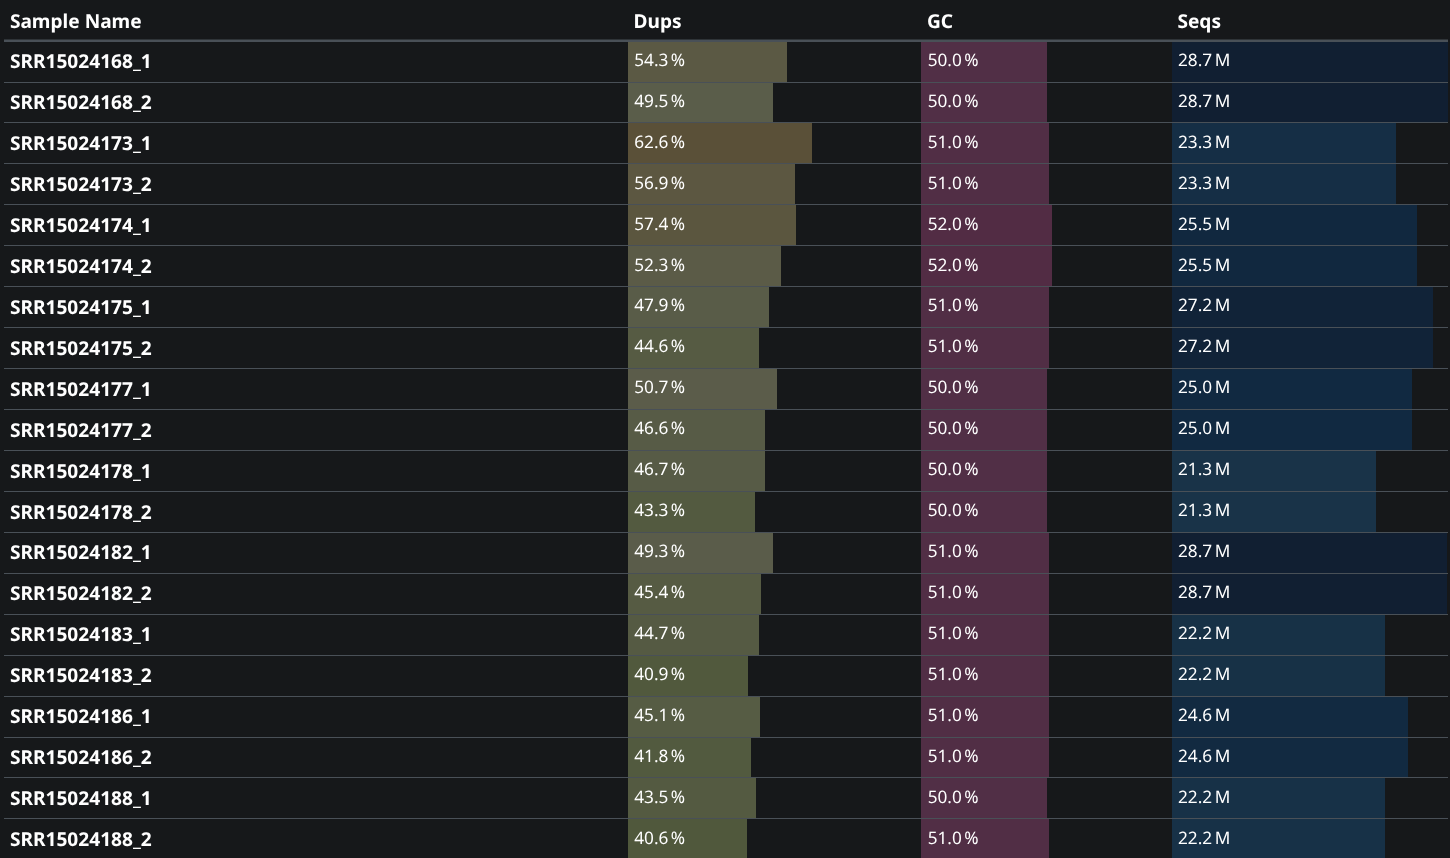
\includegraphics[width=0.5\linewidth,height=\textheight,keepaspectratio]{./data/images/multiqc/multiqc_general_stats_table_raw.png}

}

\caption{Estadísticas generales de calidad de datos crudos}

\end{figure}%

\begin{figure}[H]

{\centering 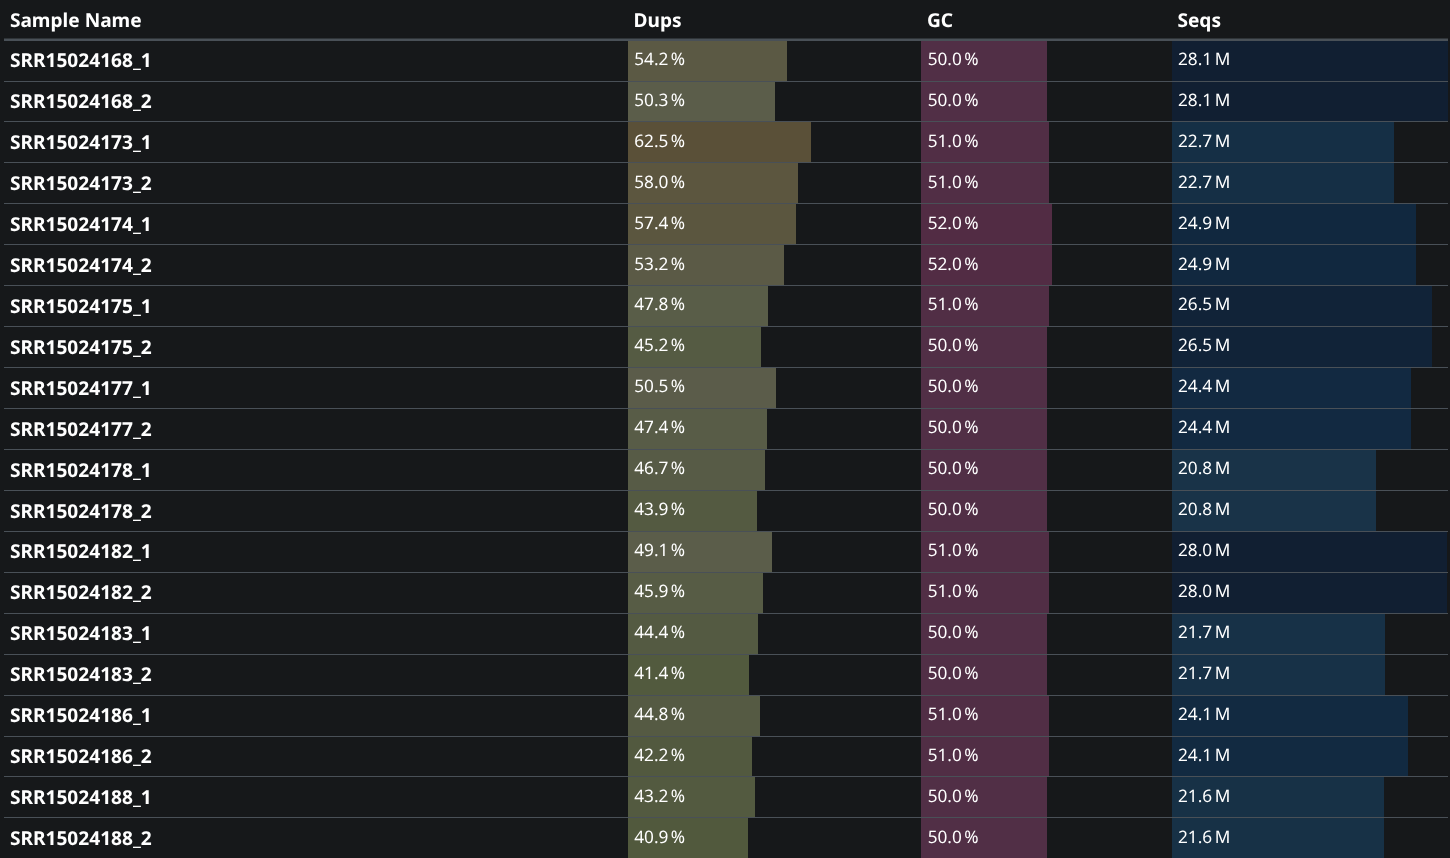
\includegraphics[width=0.5\linewidth,height=\textheight,keepaspectratio]{./data/images/multiqc/multiqc_general_stats_table_cleaned.png}

}

\caption{Estadísticas generales de calidad de datos limpios}

\end{figure}%

\begin{figure}[H]

{\centering 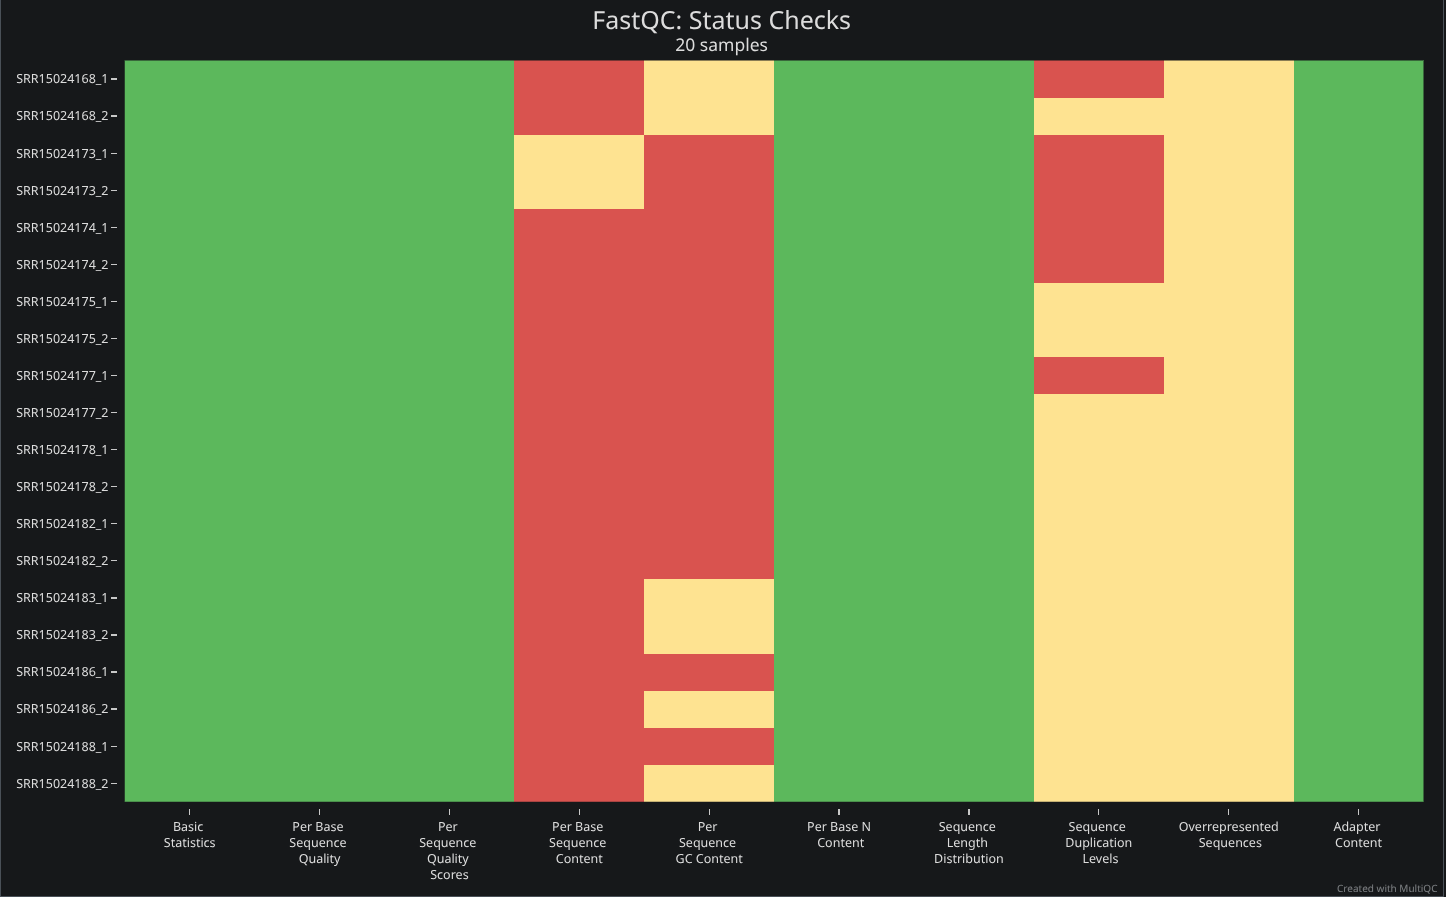
\includegraphics[width=0.5\linewidth,height=\textheight,keepaspectratio]{./data/images/multiqc/multiqc_status_check_heatmap_raw.png}

}

\caption{Heatmap de estado de calidad de datos crudos}

\end{figure}%

\begin{figure}[H]

{\centering 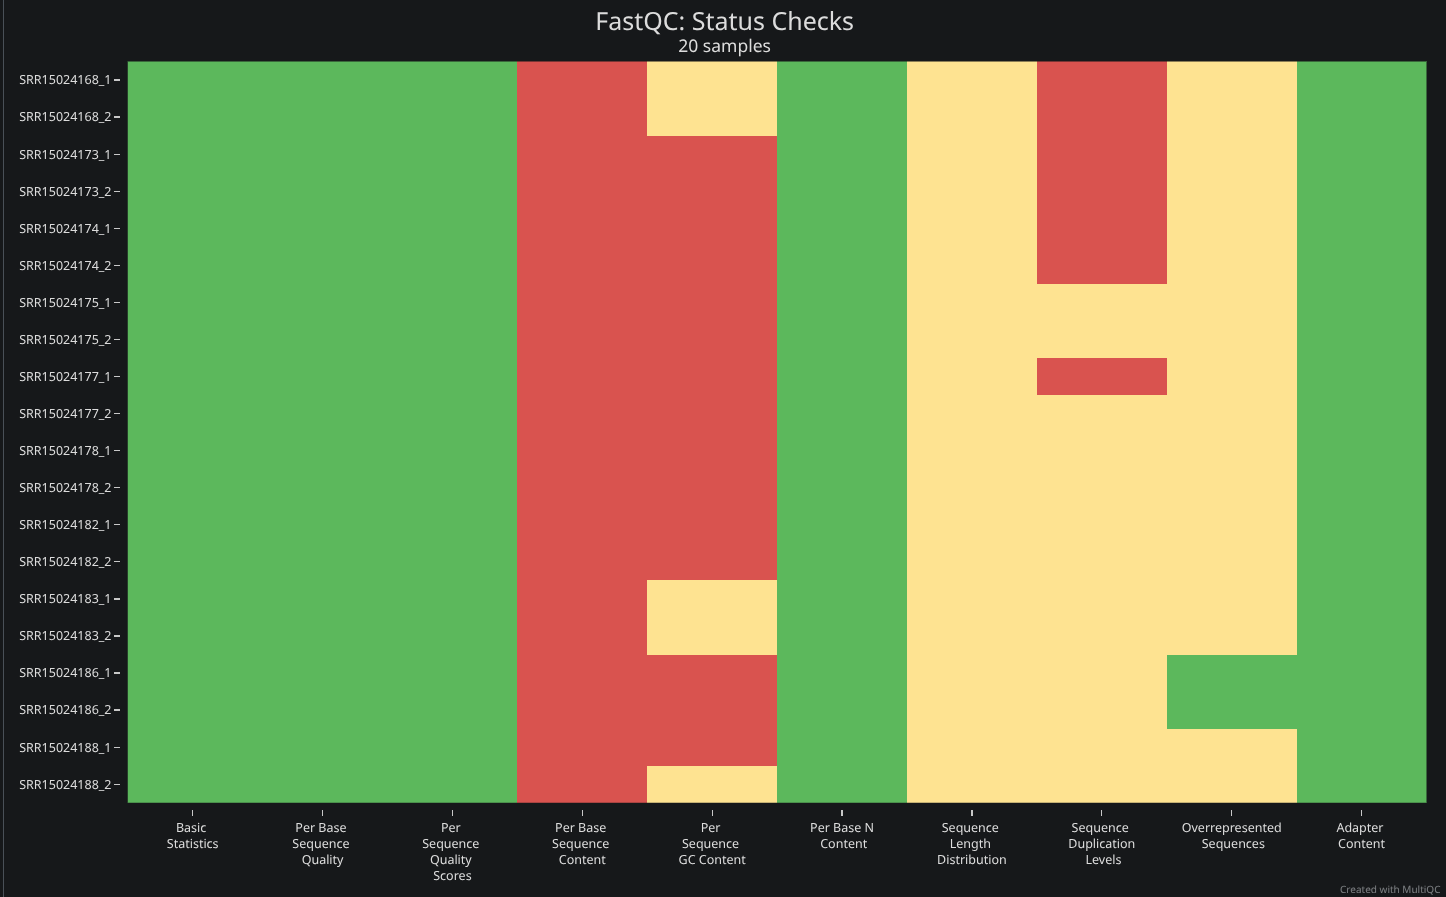
\includegraphics[width=0.5\linewidth,height=\textheight,keepaspectratio]{./data/images/multiqc/multiqc_status_check_heatmap_cleaned.png}

}

\caption{Heatmap de estado de calidad de datos limpios}

\end{figure}%

\begin{figure}[H]

{\centering 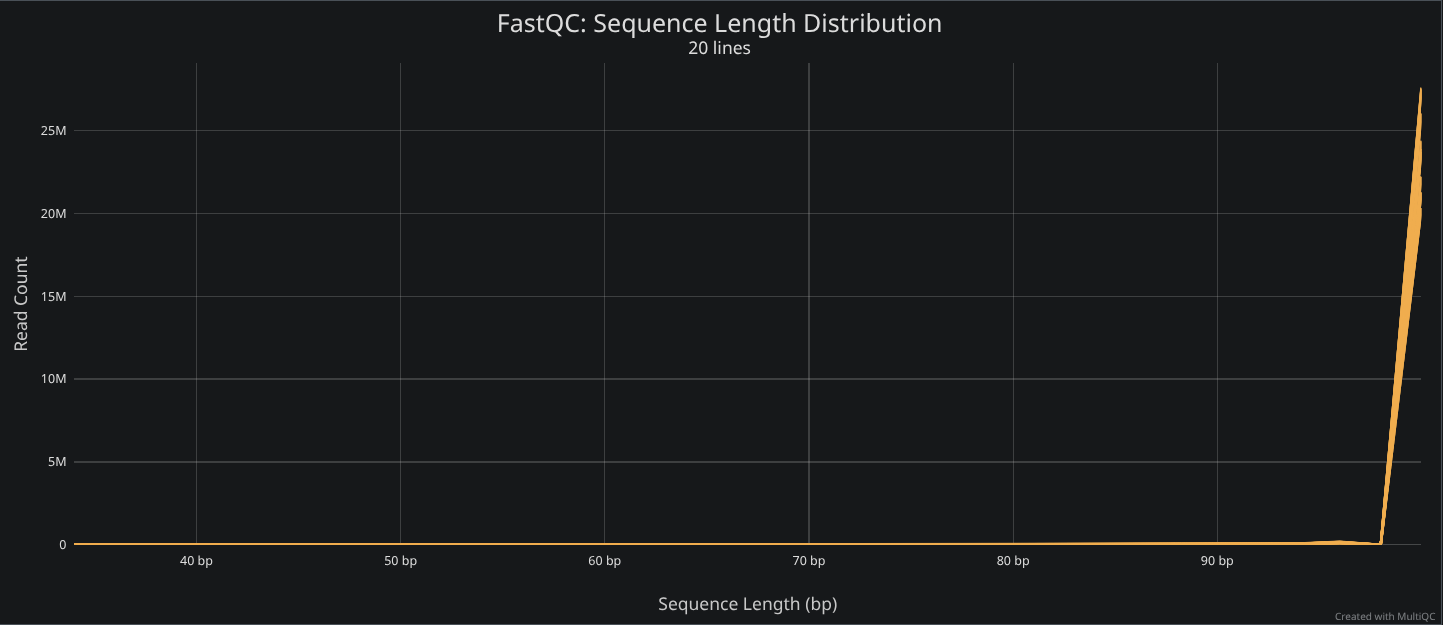
\includegraphics[width=0.5\linewidth,height=\textheight,keepaspectratio]{./data/images/multiqc/multiqc_sequence_length_distribution_cleaned.png}

}

\caption{Distribución de longitud de secuencias de datos limpios. Las
muestras pasan de medir todas 101bp a longitudes variables menores a
esta tras la limpieza. No se cuenta con la gráfica análoga de las
muestras crudas dadas las longitudes iguales}

\end{figure}%

\begin{figure}[H]

{\centering 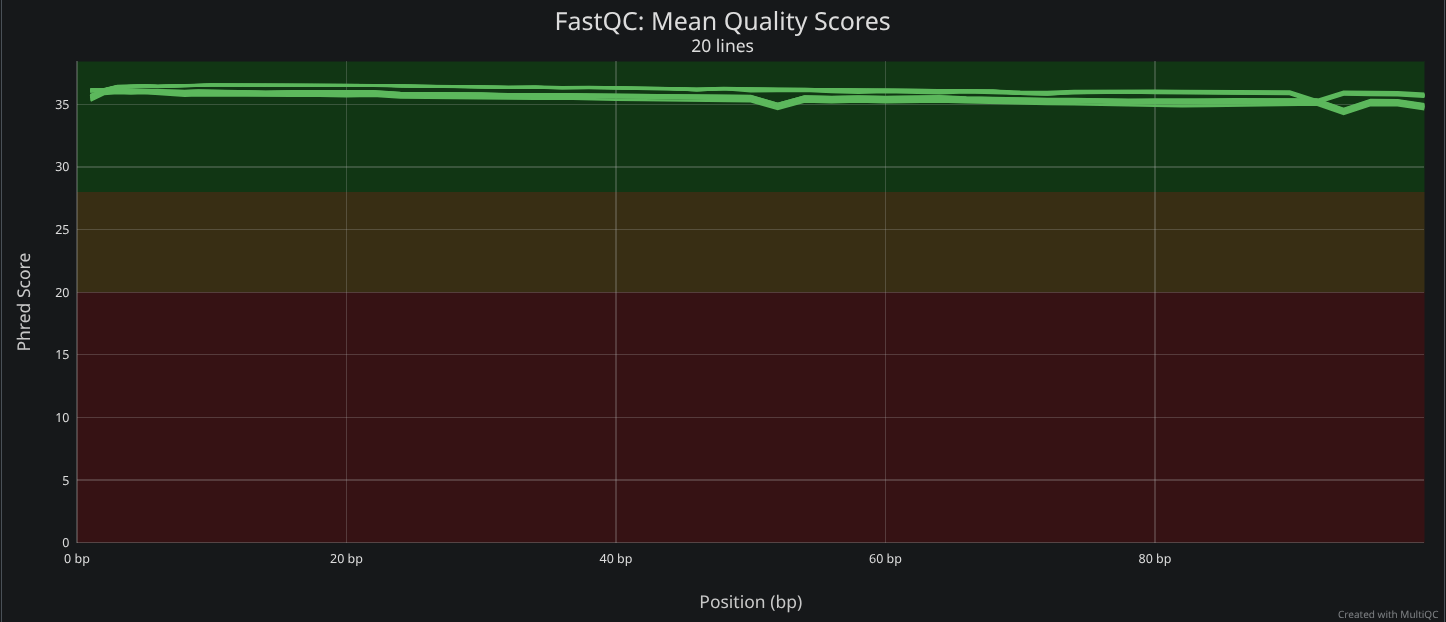
\includegraphics[width=0.5\linewidth,height=\textheight,keepaspectratio]{./data/images/multiqc/multiqc_mean_quality_scores_raw.png}

}

\caption{Calidad media de los datos crudos. Se muestra una calidad alta,
con Phred-scores mayoritariamente por encima de 35}

\end{figure}%

\begin{figure}[H]

{\centering 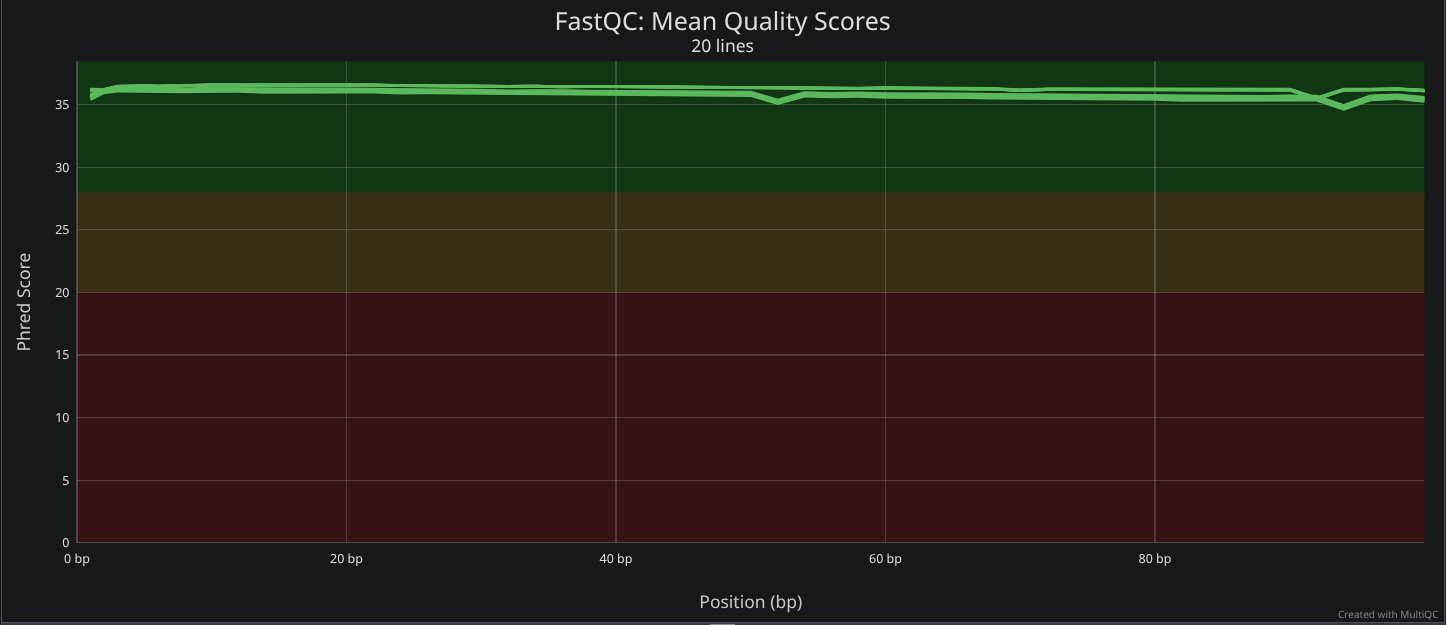
\includegraphics[width=0.5\linewidth,height=\textheight,keepaspectratio]{./data/images/multiqc/multiqc_mean_quality_scores_cleaned.png}

}

\caption{Calidad media de los datos limpios. Se mantiene una calidad
alta, con Phred-scores igualmente por encima de 35}

\end{figure}%

\subsection{Alineamientos}\label{alineamientos-1}

Se construyó también el índice de \texttt{Salmon} pero, con base en las
comparaciones realizadas en las tareas del curso y tras obtener tasas de
mapeo altas en \texttt{STAR} y \texttt{HISAT2} (alineamientos hechos
simultáneamente), se optó por no realizar \emph{pseudoalineamientos}.
Este requería, en lugar del genoma de referencia, un índice construido a
partir de las secuencias de transcritos, también obtenidas de Ensembl
{[}9,23{]}.

Se usó el siguiente \emph{script} para la conversión de \texttt{SAM} a
\texttt{BAM} de los resultados de \texttt{HISAT2}

Se generó un \emph{dataframe} con las estadísticas de alineamiento de
ambos programas con el \emph{script} \texttt{./scripts/stats\_table.py},
a partir de una estrategia híbrida de extracción de los resúmenes de
alineamiento (\texttt{*.out} para \texttt{STAR} y \texttt{*.txt} para
\texttt{HISAT2}), para extraer las tasas de mapeo único, y de los
\texttt{BAM}s con \texttt{Samtools\ flagstat}, para las métricas básicas
restantes {[}10{]}.

\subsubsection{STAR}\label{star}

\texttt{./scripts/star\_align.sh}

\subsubsection{Hisat2}\label{hisat2-1}

\begin{quote}
\texttt{HISAT2} no tiene un entorno de \emph{Conda} propio.
\end{quote}

Se utilizó \texttt{./scripts/hisat2\_align.sh}.

\subsubsection{flagstat y estadísticas de
alineamiento}\label{flagstat-y-estaduxedsticas-de-alineamiento}

\begin{table}[H]

\caption{\label{tbl-alignment-stats}Muestras jóvenes seleccionadas para
el análisis transcriptómico y sus estadísticas de alineamiento.}

\centering{

\begin{verbatim}
         Sample    Tool  ... Properly paired (%)  Unique mapping (%)
0   SRR15024173  HISAT2  ...               88.84               82.58
1   SRR15024168  HISAT2  ...               89.67               82.80
2   SRR15024174  HISAT2  ...               88.89               83.00
3   SRR15024175  HISAT2  ...               89.41               80.74
4   SRR15024178  HISAT2  ...               88.90               81.59
5   SRR15024177  HISAT2  ...               89.30               81.76
6   SRR15024183  HISAT2  ...               90.23               82.29
7   SRR15024182  HISAT2  ...               89.99               83.47
8   SRR15024186  HISAT2  ...               90.60               84.09
9   SRR15024188  HISAT2  ...               89.61               80.67
10  SRR15024168    STAR  ...               95.22               88.02
11  SRR15024173    STAR  ...               94.79               88.39
12  SRR15024174    STAR  ...               94.77               88.72
13  SRR15024175    STAR  ...               94.93               85.67
14  SRR15024177    STAR  ...               95.02               87.10
15  SRR15024178    STAR  ...               94.20               86.89
16  SRR15024182    STAR  ...               95.46               88.62
17  SRR15024183    STAR  ...               95.62               87.07
18  SRR15024188    STAR  ...               95.22               85.63
19  SRR15024186    STAR  ...               96.14               89.12

[20 rows x 11 columns]
\end{verbatim}

}

\end{table}%

\subsection{FeatureCounts}\label{featurecounts}

\begin{Shaded}
\begin{Highlighting}[]
\VariableTok{SCRIPT}\OperatorTok{=}\StringTok{"./scripts/make\_featureCounts.sh"}
\VariableTok{ALIGN\_PATH}\OperatorTok{=}\StringTok{"./results/aligned"}
\VariableTok{GTF}\OperatorTok{=}\StringTok{"./data/references/Macaca\_mulatta.Mmul\_10.115.gtf"}

\CommentTok{\# Barrido de tipo de librería}
\ControlFlowTok{for}\NormalTok{ i }\KeywordTok{in} \DataTypeTok{\{}\DecValTok{0}\DataTypeTok{..}\DecValTok{2}\DataTypeTok{\}}\KeywordTok{;} \ControlFlowTok{do}
  \ExtensionTok{qsub} \StringTok{"}\VariableTok{$SCRIPT}\StringTok{"} \StringTok{"}\VariableTok{$\{ALIGN\_PATH\}}\StringTok{/hisat2\_PE"} \StringTok{"}\VariableTok{$GTF}\StringTok{"} \StringTok{"}\VariableTok{$i}\StringTok{"}
  \ExtensionTok{qsub} \StringTok{"}\VariableTok{$SCRIPT}\StringTok{"} \StringTok{"}\VariableTok{$\{ALIGN\_PATH\}}\StringTok{/star\_PE"} \StringTok{"}\VariableTok{$GTF}\StringTok{"} \StringTok{"}\VariableTok{$i}\StringTok{"}
\ControlFlowTok{done}
\end{Highlighting}
\end{Shaded}

Resultados:

\begin{Shaded}
\begin{Highlighting}[]
\NormalTok{path }\OperatorTok{=} \StringTok{"./results/aligned/hisat2\_PE/"}

\KeywordTok{def}\NormalTok{ load\_fc\_counts(path) }\OperatorTok{{-}\textgreater{}}\NormalTok{ pd.DataFrame:}
  \ControlFlowTok{return}\NormalTok{ pd.read\_csv(path, sep}\OperatorTok{=}\StringTok{"}\CharTok{\textbackslash{}t}\StringTok{"}\NormalTok{, comment}\OperatorTok{=}\StringTok{"\#"}\NormalTok{, engine}\OperatorTok{=}\StringTok{"python"}\NormalTok{)}

\NormalTok{fc\_dfs }\OperatorTok{=}\NormalTok{ \{\}}
\CommentTok{\# Leer cada archivo de conteos}
\ControlFlowTok{for}\NormalTok{ strand }\KeywordTok{in} \BuiltInTok{range}\NormalTok{(}\DecValTok{3}\NormalTok{): }\CommentTok{\# 0, 1, 2 para los tipos de strand}
  \ControlFlowTok{for}\NormalTok{ aligner }\KeywordTok{in}\NormalTok{ [}\StringTok{"hisat2\_PE"}\NormalTok{, }\StringTok{"star\_PE"}\NormalTok{]:}
\NormalTok{    fc\_dfs[}\SpecialStringTok{f"fc\_}\SpecialCharTok{\{}\NormalTok{aligner}\SpecialCharTok{\}}\SpecialStringTok{\_}\SpecialCharTok{\{}\NormalTok{strand}\SpecialCharTok{\}}\SpecialStringTok{"}\NormalTok{] }\OperatorTok{=}\NormalTok{ (df }\OperatorTok{:=}\NormalTok{ load\_fc\_counts(}\SpecialStringTok{f"./results/aligned/}\SpecialCharTok{\{}\NormalTok{aligner}\SpecialCharTok{\}}\SpecialStringTok{/counts\_per\_gene\_}\SpecialCharTok{\{}\NormalTok{strand}\SpecialCharTok{\}}\SpecialStringTok{.txt"}\NormalTok{))}
    \BuiltInTok{print}\NormalTok{(}\SpecialStringTok{f"}\SpecialCharTok{\{}\NormalTok{aligner}\SpecialCharTok{\}}\SpecialStringTok{ y strandness }\SpecialCharTok{\{}\NormalTok{strand}\SpecialCharTok{\}}\SpecialStringTok{:"}\NormalTok{)}
    \BuiltInTok{print}\NormalTok{(df.head())}
\end{Highlighting}
\end{Shaded}

\begin{verbatim}
hisat2_PE y strandness 0:
               Geneid  ... ./results/aligned/hisat2_PE/SRR15024188.fs.bam
0  ENSMMUG00000023296  ...                                              0
1  ENSMMUG00000036181  ...                                              1
2  ENSMMUG00000000634  ...                                            622
3  ENSMMUG00000037875  ...                                            238
4  ENSMMUG00000000632  ...                                           2003

[5 rows x 16 columns]
star_PE y strandness 0:
               Geneid  ... ./results/aligned/star_PE/SRR15024188_Aligned.sortedByCoord.out.fs.bam
0  ENSMMUG00000023296  ...                                                  0                    
1  ENSMMUG00000036181  ...                                                  1                    
2  ENSMMUG00000000634  ...                                                673                    
3  ENSMMUG00000037875  ...                                                252                    
4  ENSMMUG00000000632  ...                                               2083                    

[5 rows x 16 columns]
hisat2_PE y strandness 1:
               Geneid  ... ./results/aligned/hisat2_PE/SRR15024188.fs.bam
0  ENSMMUG00000023296  ...                                              0
1  ENSMMUG00000036181  ...                                              1
2  ENSMMUG00000000634  ...                                            557
3  ENSMMUG00000037875  ...                                            331
4  ENSMMUG00000000632  ...                                           1056

[5 rows x 16 columns]
star_PE y strandness 1:
               Geneid  ... ./results/aligned/star_PE/SRR15024188_Aligned.sortedByCoord.out.fs.bam
0  ENSMMUG00000023296  ...                                                  0                    
1  ENSMMUG00000036181  ...                                                  1                    
2  ENSMMUG00000000634  ...                                                586                    
3  ENSMMUG00000037875  ...                                                337                    
4  ENSMMUG00000000632  ...                                               1079                    

[5 rows x 16 columns]
hisat2_PE y strandness 2:
               Geneid  ... ./results/aligned/hisat2_PE/SRR15024188.fs.bam
0  ENSMMUG00000023296  ...                                              0
1  ENSMMUG00000036181  ...                                              0
2  ENSMMUG00000000634  ...                                            598
3  ENSMMUG00000037875  ...                                            336
4  ENSMMUG00000000632  ...                                            973

[5 rows x 16 columns]
star_PE y strandness 2:
               Geneid  ... ./results/aligned/star_PE/SRR15024188_Aligned.sortedByCoord.out.fs.bam
0  ENSMMUG00000023296  ...                                                  0                    
1  ENSMMUG00000036181  ...                                                  0                    
2  ENSMMUG00000000634  ...                                                630                    
3  ENSMMUG00000037875  ...                                                348                    
4  ENSMMUG00000000632  ...                                               1004                    

[5 rows x 16 columns]
\end{verbatim}

Tasas promedio de mapeo tras \texttt{featureCounts}, por tipo de
alineador y strandness:

\begin{table}[H]

\caption{\label{tbl-fc-mapping-rates}Tasas de mapeo promedio obtenidas
con \texttt{featureCounts} para cada alineador y tipo de strandness.}

\centering{

\begin{verbatim}
     aligner  strandness  mean_percentage
0  hisat2_PE           0            66.87
1  hisat2_PE           1            36.17
2  hisat2_PE           2            35.61
3    star_PE           0            71.87
4    star_PE           1            38.38
5    star_PE           2            37.80
\end{verbatim}

}

\end{table}%

\begin{verbatim}
Genes comunes entre las matrices: 35432
\end{verbatim}

\begin{verbatim}
hisat2_PE: (35432, 10)
star_PE: (35432, 10)
\end{verbatim}

\subsection{Anotaciones y archivos
auxiliares}\label{anotaciones-y-archivos-auxiliares-1}

Script de generación de tabla de correspondencia entre \texttt{gene\_id}
y \texttt{gene\_name} a partir del GTF:

\begin{table}[H]

\caption{\label{tbl-gene-id-name}Tabla de correspondencia antes de
quitar duplicados entre \texttt{gene\_id} y \texttt{gene\_name},
derivada del GTF. Se muestran los primeros registros.}

\centering{

\begin{verbatim}
Antes de quitar duplicados: (24482, 2)
\end{verbatim}

\begin{verbatim}
               Geneid Gene_name
0  ENSMMUG00000023296     PGBD2
1  ENSMMUG00000036181        U6
2  ENSMMUG00000000634    ZNF692
3  ENSMMUG00000037875    ZNF672
4  ENSMMUG00000000632   SH3BP5L
\end{verbatim}

}

\end{table}%

\begin{table}[H]

\caption{\label{tbl-gene-id-name-clean}Tabla de correspondencia después
de quitar duplicados entre \texttt{gene\_id} y \texttt{gene\_name},
derivada del GTF. Se muestran los primeros registros, con 24,482 filas.}

\centering{

\begin{verbatim}
Después de quitar duplicados: (24482, 2)
\end{verbatim}

\begin{verbatim}
               Geneid Gene_name
0  ENSMMUG00000023296     PGBD2
1  ENSMMUG00000036181        U6
2  ENSMMUG00000000634    ZNF692
3  ENSMMUG00000037875    ZNF672
4  ENSMMUG00000000632   SH3BP5L
\end{verbatim}

}

\end{table}%

Para la tabla de longitudes génicas se utilizan las longitudes
reportadas por \texttt{featureCounts} para cada gen (\texttt{Geneid}) en
la columna \texttt{Length} de sus tablas de conteo, que corresponden a
su vez a la suma de las longitudes de los exones de cada gen en la
anotación del GTF {[}11{]}:

\begin{quote}
Dado que el GTF es el mismo para ambos alineamientos, se utiliza el
archivo de \texttt{featureCounts} de \texttt{star}
(\texttt{./results/aligned/star/counts\_per\_gene.txt}).
\end{quote}

La generación de ortólogos se realiza a través de la función
\texttt{homologene} del paquete \texttt{homologene} de Bioconductor, que
consulta la base de datos de HomoloGene para encontrar genes ortólogos
entre especies {[}17{]}. Se parte de los símbolos génicos
(\texttt{gene\_name}) presentes en las matrices de conteos, se
convierten a símbolos humanos utilizando \texttt{org.Hs.eg.db} y luego
se obtiene la tabla de correspondencia entre los símbolos de macaco y
humano. Finalmente, se exporta esta tabla para su uso en el análisis de
enriquecimiento funcional.

\subsection{Tabla de condiciones}\label{tabla-de-condiciones}

Se utiliza nuevamente la matriz de \texttt{star\_PE} para obtener el
orden de las muestras, dado que este es consistente a lo largo de todas
las matrices.

\subsection{Pipeline de expresión
diferencial}\label{pipeline-de-expresiuxf3n-diferencial}

\begin{figure}[H]

{\centering 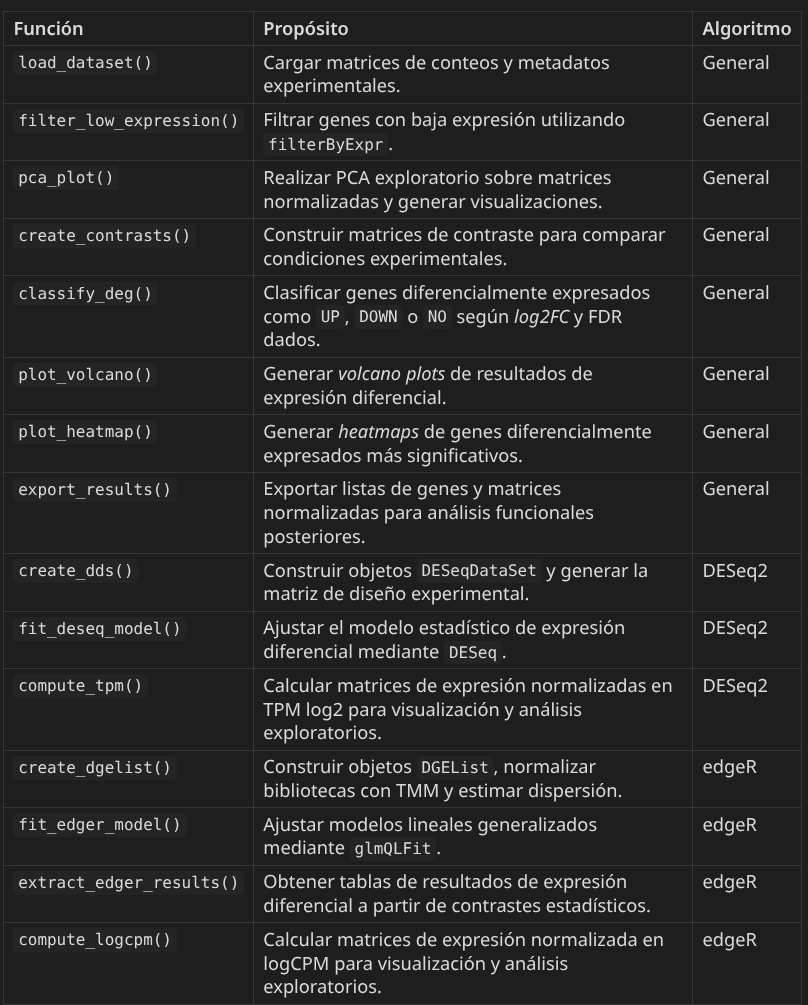
\includegraphics[width=0.5\linewidth,height=\textheight,keepaspectratio]{./data/images/table_funciones_de.png}

}

\caption{Funciones implementadas en el pipeline de análisis
transcriptómico, incluyendo utilidades generales de preprocesamiento,
visualización y exportación, así como funciones específicas para
análisis de expresión diferencial con DESeq2 y edgeR.}

\end{figure}%

\subsubsection{Carga de datos}\label{carga-de-datos}

\subsubsection{Funciones generales}\label{funciones-generales}

Se definen las funciones reutilizables para ambos algoritmos, buscando
máxima comparabilidad entre los métodos:

\paragraph{Cargado de matriz}\label{cargado-de-matriz}

\paragraph{Filtrado de genes}\label{filtrado-de-genes}

\paragraph{PCA exploratorio}\label{pca-exploratorio}

Mostrando la varianza de todos los genes:

Mostrando la varianza del top n genes que más presentan:

\paragraph{Volcano plot y heatmap}\label{volcano-plot-y-heatmap}

\subsubsection{Exportar resultados}\label{exportar-resultados}

\subsubsection{Funciones de DESeq2}\label{funciones-de-deseq2}

En general, las funciones de \texttt{DESeq2} son de alto nivel. Aún así,
se definieron funciones específicas por simplicidad y en aras de
mantener un flujo de análisis homogéneo entre los métodos.

\paragraph{Ajuste del modelo}\label{ajuste-del-modelo}

\paragraph{Normalización a TPM}\label{normalizaciuxf3n-a-tpm}

\subsubsection{edgeR}\label{edger}

\paragraph{DGEList}\label{dgelist}

En \texttt{edgeR} se usa \texttt{DGEList}, que se crea a partir de la
matriz de conteos, los metadatos y el diseño experimental. De acuerdo al
flujo, se define una función específica para su construcción
{[}13,24{]}. Asimismo, se integran en la función los procesos de
normalización de bibliotecas mediante TMM (Trimmed Mean of M-values) con
\texttt{calcNormFactors}, para corregir diferencias de composición y
profundidad; y la estimación de dispersión con \texttt{estimateDisp},
para modelar la sobredispersión de los conteos. Estos, en contraposición
con \texttt{DESeq2}, se realizan de forma explícita {[}13{]}.

\paragraph{Ajuste de modelo}\label{ajuste-de-modelo}

El ajuste del modelo de DE se realiza con la función \texttt{glmQLFit},
renombrada \texttt{fit\_edger\_model}. Esta ajusta un modelo lineal
generalizado con el método \emph{cuasilikelihood}, permitiendo así
modelar la variabilidad adicional presente en los datos de
\emph{RNA-seq} {[}13{]}. La función recibe el objeto \texttt{DGEList} y
la matriz de diseño experimental, y devuelve un objeto con el modelo
ajustado listo para realizar los contrastes de expresión diferencial.

\paragraph{Extracción de resultados}\label{extracciuxf3n-de-resultados}

Se utiliza la función \texttt{glmQLFTest} para realizar los contrastes
de DE. Esta toma como input el modelo ajustado y la matriz de contrastes
generada. Regresa una tabla con los resultados de DE, incluyendo
\emph{Log2 fold-change} y FDR ajustado.

\paragraph{logCPM}\label{logcpm}

Para los análisis exploratorios y visualizaciones en \texttt{edgeR}, se
utiliza una matriz transformada a logCPM (\emph{log Counts Per Million})
por la función \texttt{cpm}. Esta métrica normaliza los conteos según el
tamaño de biblioteca y aplica una transformación logarítmica,
permitiendo reducir parcialmente la heterocedasticidad inherente a los
datos {[}13,24{]}.

\paragraph{Implementación}\label{implementaciuxf3n}

\subsection{PCAs}\label{pcas}

\begin{figure}[H]

{\centering 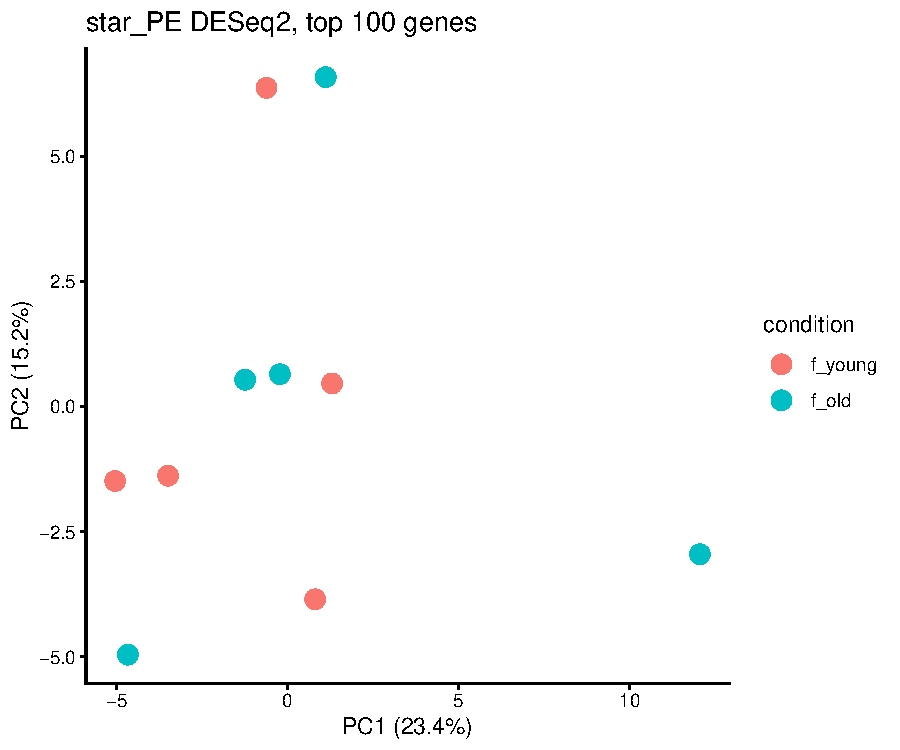
\includegraphics[width=0.5\linewidth,height=\textheight,keepaspectratio]{./results/plots/deseq2/pca/star_PE_pca_top100.pdf}

}

\caption{PCA de muestras analizadas con DESeq2 y STAR utilizando los 250
genes con mayor varianza. El análisis se realizó sobre la matriz de
expresión normalizada en TPM log2, priorizando genes con mayor
variabilidad entre muestras para facilitar la visualización de patrones
globales de expresión.}

\end{figure}%

\begin{figure}[H]

{\centering 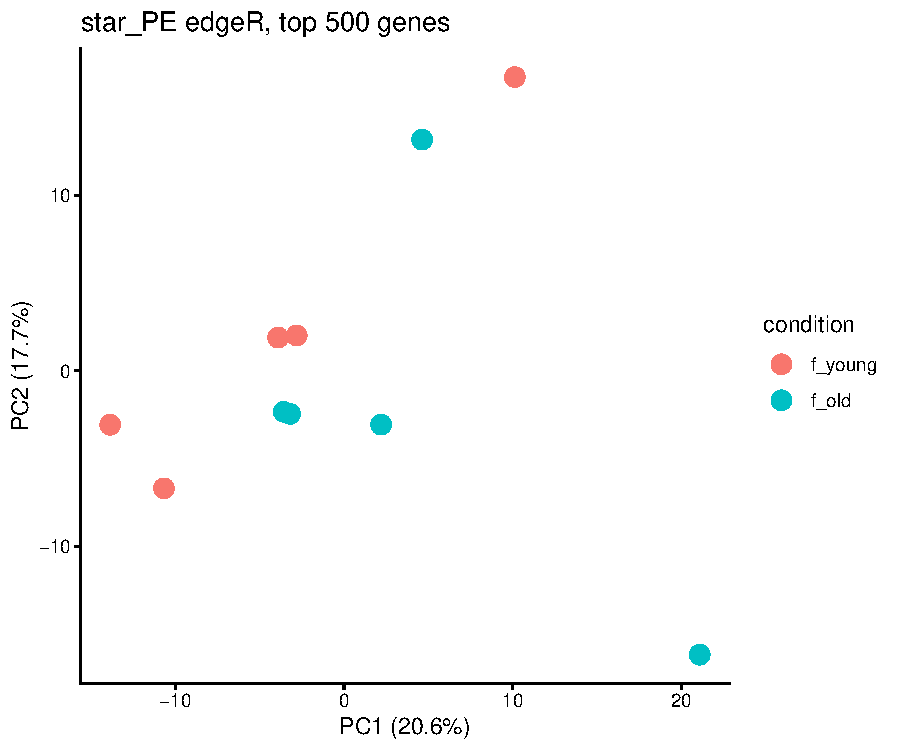
\includegraphics[width=0.5\linewidth,height=\textheight,keepaspectratio]{./results/plots/edger/pca/star_PE_pca_top500.pdf}

}

\caption{PCA de muestras analizadas con edgeR y STAR utilizando los 500
genes con mayor varianza. El análisis se realizó sobre la matriz de
expresión normalizada en logCPM para enfatizar las principales fuentes
de variación transcriptómica entre las muestras.}

\end{figure}%

\begin{figure}[H]

{\centering 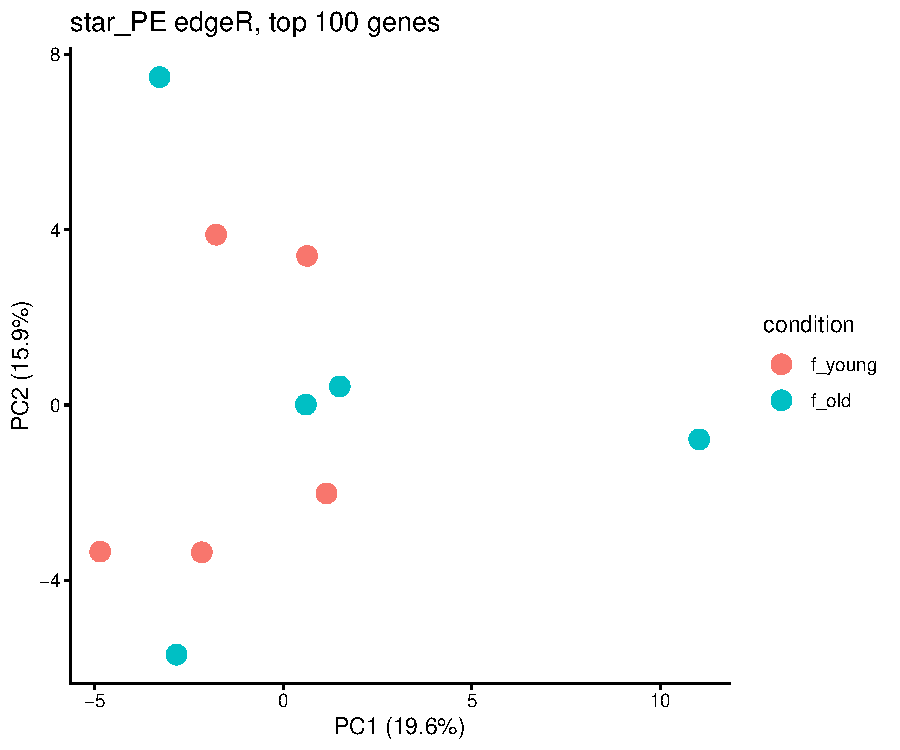
\includegraphics[width=0.5\linewidth,height=\textheight,keepaspectratio]{./results/plots/edger/pca/star_PE_pca_top100.pdf}

}

\caption{PCA de muestras analizadas con edgeR y STAR utilizando los 250
genes con mayor varianza. El análisis se realizó sobre la matriz de
expresión normalizada en logCPM priorizando genes altamente variables
para facilitar la identificación de patrones globales de agrupamiento.}

\end{figure}%

\begin{figure}[H]

{\centering 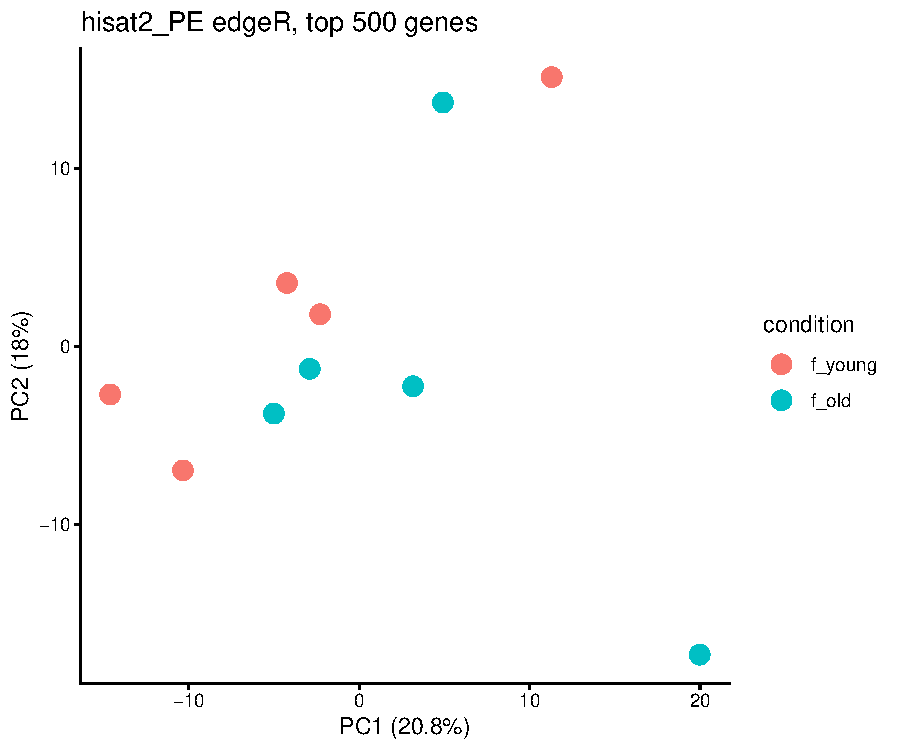
\includegraphics[width=0.5\linewidth,height=\textheight,keepaspectratio]{./results/plots/edger/pca/hisat2_PE_pca_top500.pdf}

}

\caption{PCA de muestras analizadas con edgeR y HISAT2 utilizando los
500 genes con mayor varianza. El análisis se realizó sobre la matriz de
expresión normalizada en logCPM para enfatizar las principales fuentes
de variación transcriptómica entre muestras.}

\end{figure}%

\begin{figure}[H]

{\centering 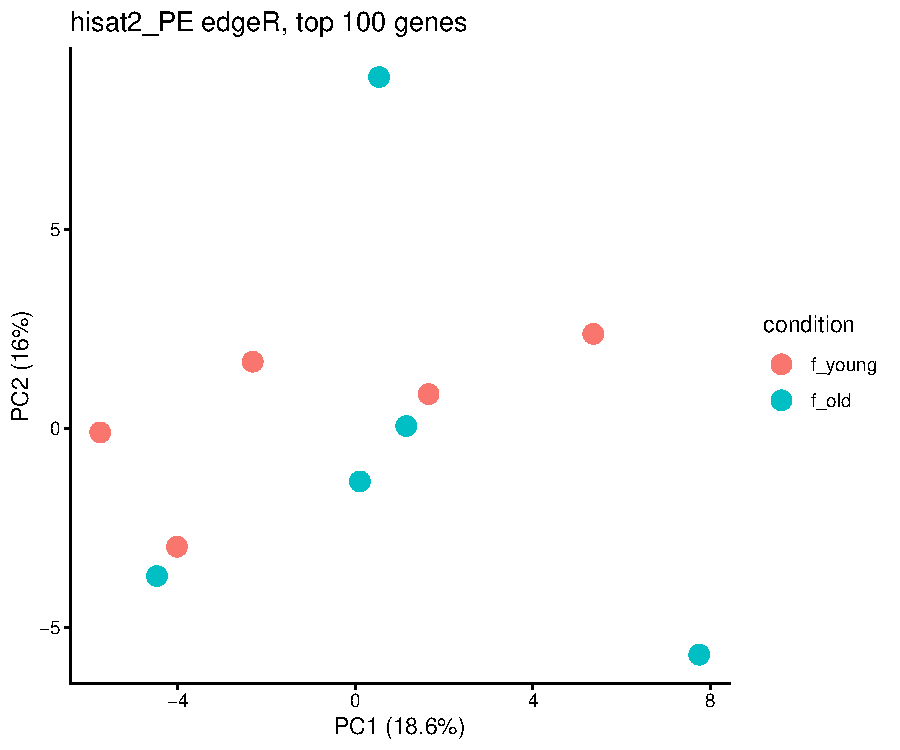
\includegraphics[width=0.5\linewidth,height=\textheight,keepaspectratio]{./results/plots/edger/pca/hisat2_PE_pca_top100.pdf}

}

\caption{PCA de muestras analizadas con edgeR y HISAT2 utilizando los
250 genes con mayor varianza. El análisis se realizó sobre la matriz de
expresión normalizada en logCPM priorizando genes altamente variables
para facilitar la visualización de patrones globales de agrupamiento
entre condiciones.}

\end{figure}%

\subsection{Heatmaps}\label{heatmaps}

\begin{figure}[H]

{\centering 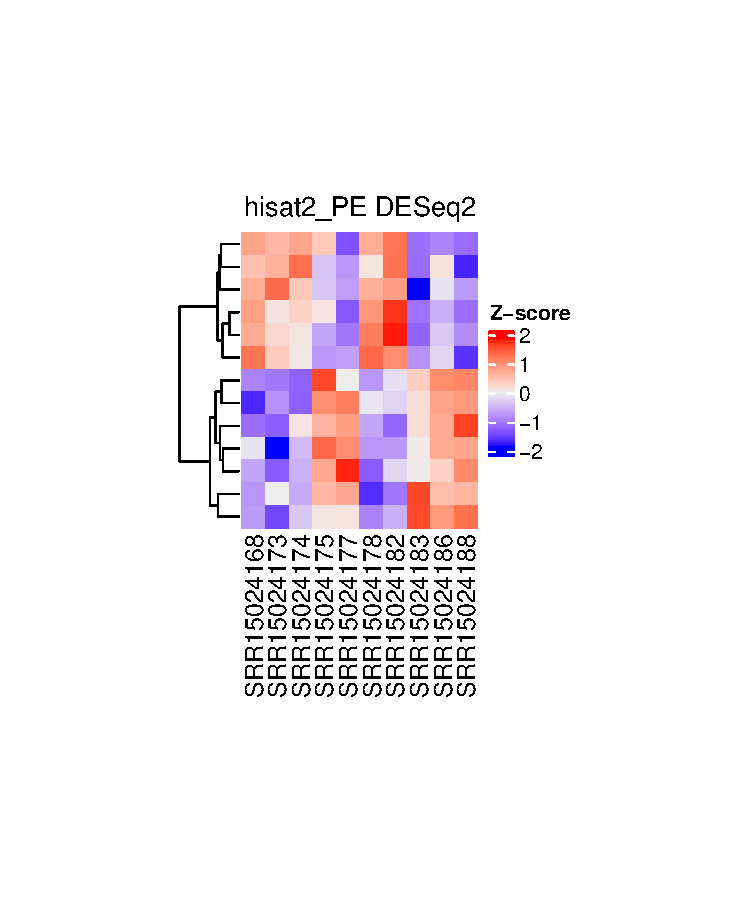
\includegraphics[width=0.5\linewidth,height=\textheight,keepaspectratio]{./results/plots/deseq2/heatmap/hisat2_PE_heatmap.pdf}

}

\caption{Heatmap de los genes diferencialmente expresados más
significativos obtenidos con DESeq2 a partir de alineamientos realizados
con HISAT2. Se muestran niveles de expresión normalizados en TPM log2
transformados a Z-score por gen. Los patrones generales son concordantes
con los obtenidos mediante STAR.}

\end{figure}%

\subsection{Volcano plots}\label{volcano-plots}

\begin{figure}[H]

{\centering 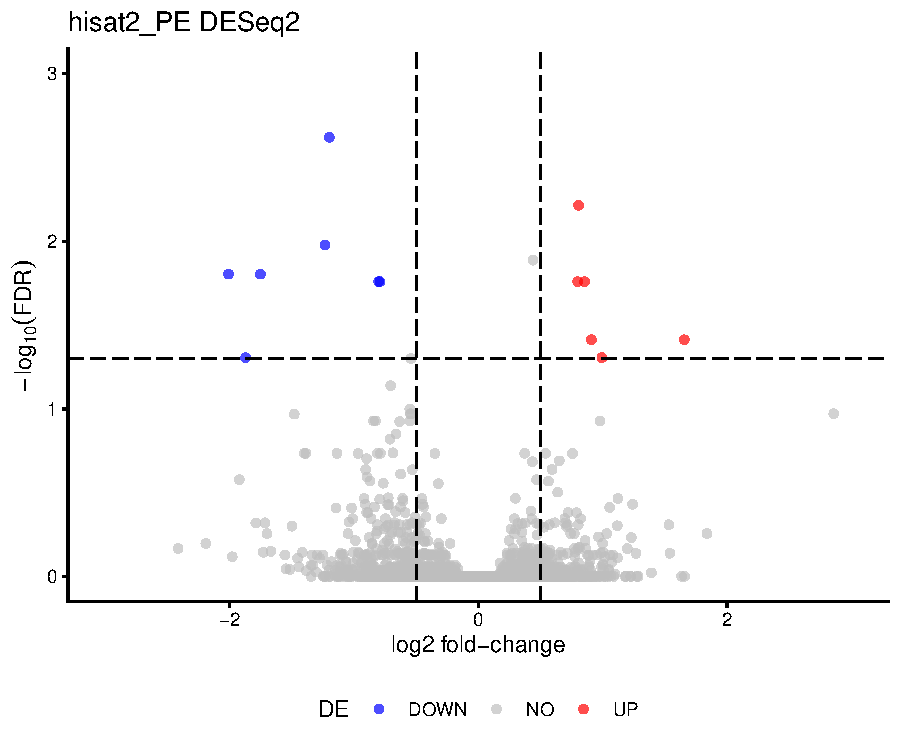
\includegraphics[width=0.5\linewidth,height=\textheight,keepaspectratio]{./results/plots/deseq2/volcano/hisat2_PE_volcano.pdf}

}

\caption{Volcano plot de genes diferencialmente expresados obtenidos con
DESeq2 a partir de alineamientos realizados con HISAT2. Se muestran los
valores de log2 fold-change frente a −log10(FDR), utilizando como
criterios de significancia \textbar log2FC\textbar{} \textgreater{} 0.5
y FDR \textless{} 0.05.}

\end{figure}%

\subsection{Enriquecimiento
funcional}\label{enriquecimiento-funcional-1}

\subsubsection{DAVID}\label{david}

\paragraph{Functional Annotation
Chart}\label{functional-annotation-chart}

Por comodidad visual, se cambia el delimitador de \texttt{,} a
\texttt{\textbackslash{}t} en los archivos descargados.

\begin{quote}
El código no se muestra en el archivo renderizado pero se encuentra en
\texttt{./JimenezSotelo\_Mateo\_ProyectoFinal.qmd} para su consulta.
\end{quote}

\begin{table}[H]

\caption{\label{tbl-david}Tabla de términos enriquecidos en DAVID para
genes subexpresados con DESeq2 y STAR.}

\centering{

\begin{verbatim}
Category    Term    Count   List Total  Pop Hits    Pop Total   P-Value Benjamini   Fold Enrichment Bonferroni  FDR Fisher Exact    User Ids
UP_KW_BIOLOGICAL_PROCESS    Apoptosis   2   2   322 5516    0.0584  0.277   17.13   0.344   0.277   0.0034  IFI27,TNFRSF1A
UP_SEQ_FEATURE  TRANSMEM:Helical    3   3   2225    8778    0.0642  1.0 3.95    0.914   1.0 0.0163  MC4R,IFI27,TNFRSF1A
UP_KW_BIOLOGICAL_PROCESS    Host-virus interaction  2   2   436 5516    0.079   0.277   12.65   0.438   0.277   0.00623 IFI27,TNFRSF1A
GOTERM_BP_DIRECT    apoptotic process   2   3   383 8478    0.0883  1.0 14.76   0.997   1.0 0.00592 IFI27,TNFRSF1A
\end{verbatim}

}

\end{table}%

\paragraph{Plots David}\label{plots-david}

Se generan los \emph{plots} de los términos y los conteos asociados.

\subsubsection{GSEA}\label{gsea}

Se generan los \emph{plots} de los pathways enriquecidos, mostrando el
NES y el FDR asociado.




\end{document}
